\documentclass{article}
\usepackage{tikz}
\usepackage{amsmath}
\usetikzlibrary{positioning, arrows.meta, shapes.geometric, shadows}
\usepackage[margin=1in]{geometry}

\begin{document}

\section*{All Figures Test Compilation}

% Immune
% Figure: Normal Immune Response
% Balanced activation, clearance, and resolution

\begin{figure}[htbp]
\centering
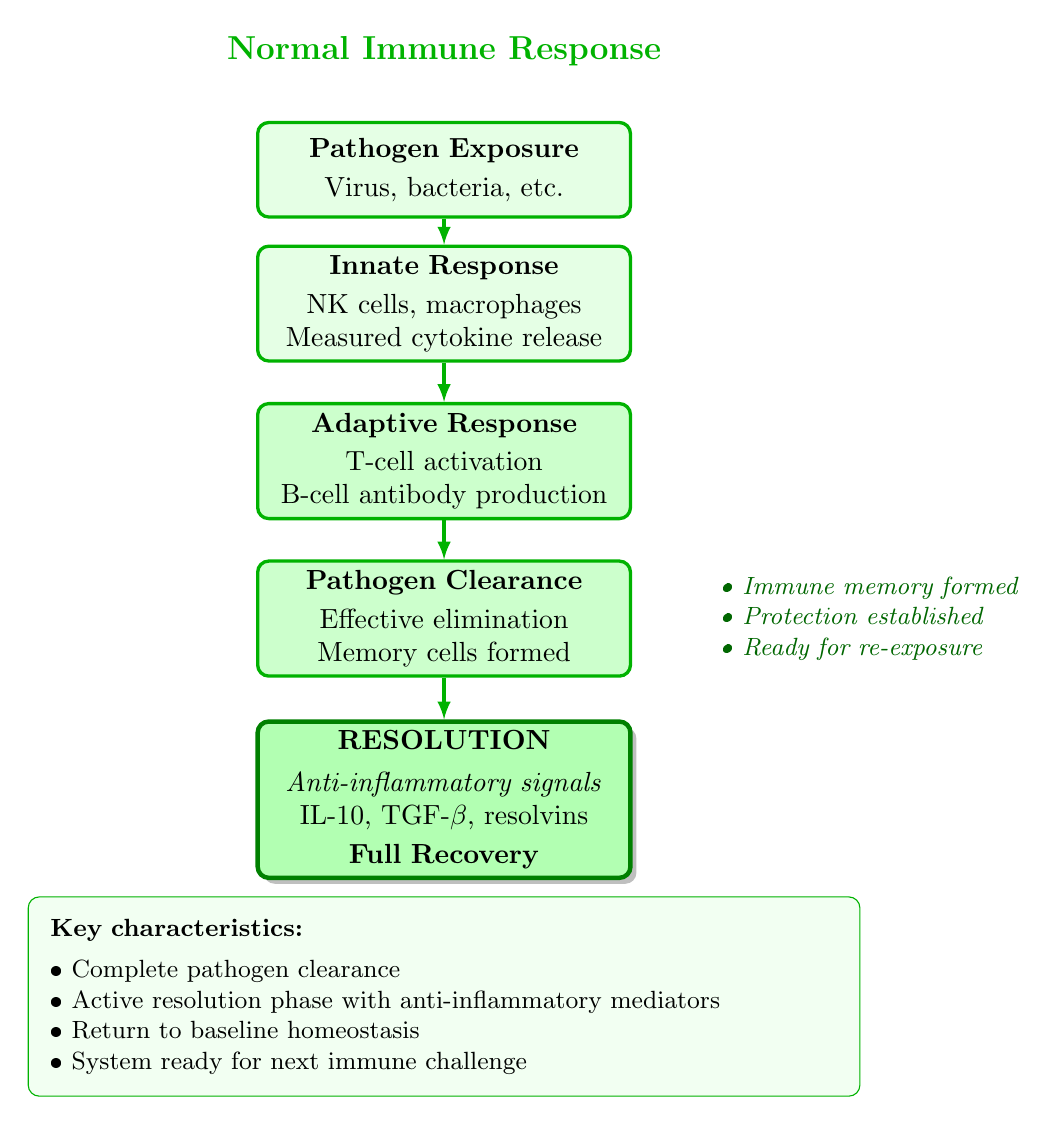
\begin{tikzpicture}[scale=1, every node/.style={scale=1},
    % Styles
    process/.style={draw=green!70!black, fill=green!10, very thick, rounded corners, text width=4.5cm, align=center, minimum height=1.2cm},
    adaptive/.style={draw=green!70!black, fill=green!20, very thick, rounded corners, text width=4.5cm, align=center, minimum height=1.2cm},
    resolution/.style={draw=green!50!black, fill=green!30, ultra thick, rounded corners, text width=4.5cm, align=center, minimum height=1.3cm, drop shadow},
    arrow/.style={-latex, very thick, green!70!black, line width=1.2pt},
    note/.style={font=\small\itshape, text width=3.8cm, align=left, green!40!black},
]

% Title
\node[font=\large\bfseries, green!70!black] at (0, 9) {Normal Immune Response};

% Pathogen exposure
\node[process] (pathogen) at (0, 7.5) {\textbf{Pathogen Exposure}\\[2pt] Virus, bacteria, etc.};

% Innate response
\node[process] (innate) at (0, 5.8) {\textbf{Innate Response}\\[2pt] NK cells, macrophages\\Measured cytokine release};
\draw[arrow] (pathogen) -- (innate);

% Adaptive response
\node[adaptive] (adaptive) at (0, 3.8) {\textbf{Adaptive Response}\\[2pt] T-cell activation\\B-cell antibody production};
\draw[arrow] (innate) -- (adaptive);

% Pathogen clearance
\node[adaptive] (clearance) at (0, 1.8) {\textbf{Pathogen Clearance}\\[2pt] Effective elimination\\Memory cells formed};
\draw[arrow] (adaptive) -- (clearance);
\node[note, right=1cm of clearance, anchor=west] {
    \textbullet~Immune memory formed\\
    \textbullet~Protection established\\
    \textbullet~Ready for re-exposure
};

% Resolution - emphasized as key success marker
\node[resolution] (resolution) at (0, -0.5) {\textbf{RESOLUTION}\\[3pt] \textit{Anti-inflammatory signals}\\IL-10, TGF-$\beta$, resolvins\\[2pt] \textbf{Full Recovery}};
\draw[arrow] (clearance) -- (resolution);

% Key point box
\node[draw=green!70!black, fill=green!5, rounded corners, text width=10cm, align=left, font=\small, inner sep=8pt] at (0, -3) {
\textbf{Key characteristics:}\\[4pt]
\textbullet~Complete pathogen clearance\\
\textbullet~Active resolution phase with anti-inflammatory mediators\\
\textbullet~Return to baseline homeostasis\\
\textbullet~System ready for next immune challenge
};

\end{tikzpicture}
\caption{Normal immune response with appropriate activation and resolution.}
\label{fig:immune-normal}
\end{figure}

\clearpage
% Figure: Immune Dysfunction in ME/CFS
% Paradoxical state: chronic inflammation but impaired function

\begin{figure}[htbp]
\centering
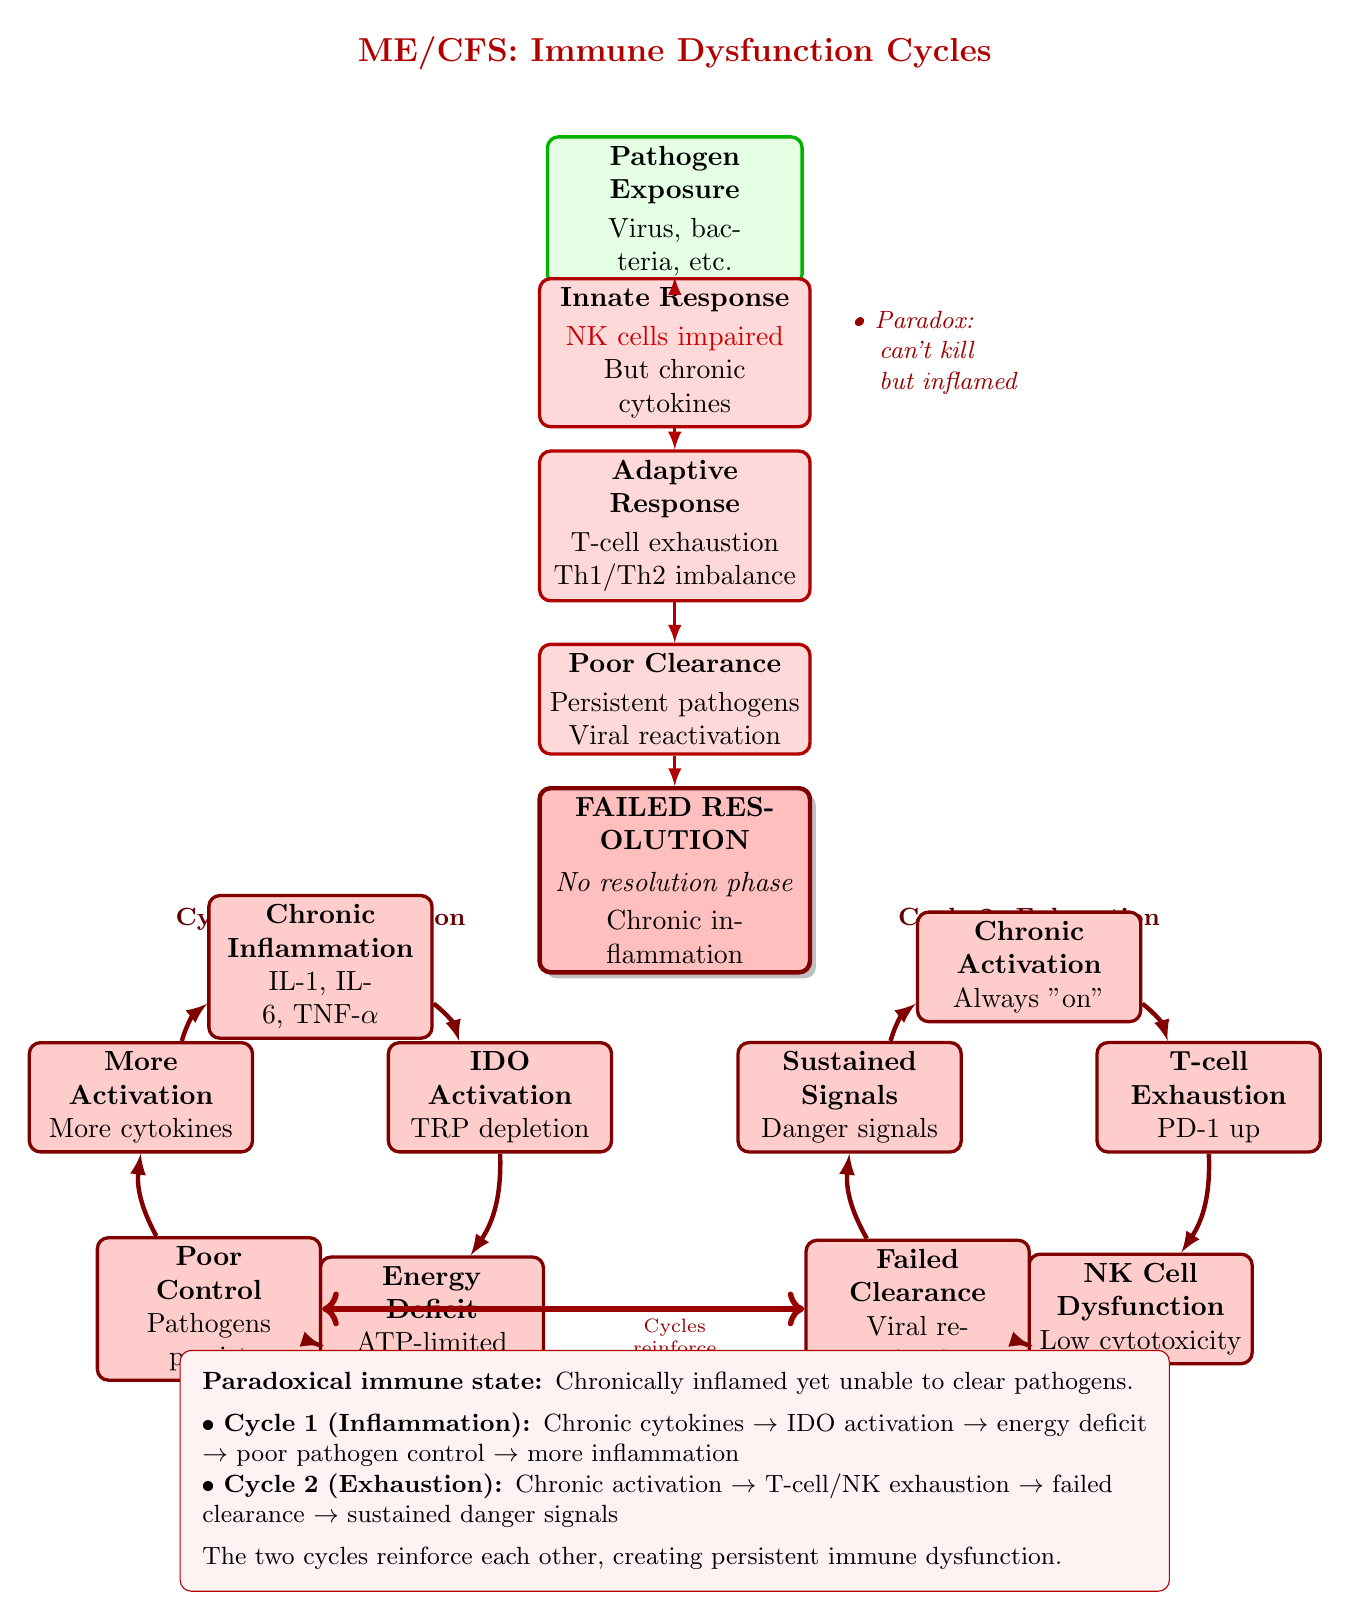
\begin{tikzpicture}[scale=1, every node/.style={scale=1},
    % Styles
    normal/.style={draw=green!70!black, fill=green!10, very thick, rounded corners, text width=3cm, align=center, minimum height=1cm},
    impaired/.style={draw=red!70!black, fill=red!15, very thick, rounded corners, text width=3.2cm, align=center, minimum height=1cm},
    severe/.style={draw=red!50!black, fill=red!25, ultra thick, rounded corners, text width=3.2cm, align=center, minimum height=1.1cm, drop shadow},
    pathological/.style={draw=red!50!black, fill=red!20, very thick, rounded corners, text width=2.6cm, align=center, minimum height=0.95cm},
    impaired-arrow/.style={-latex, very thick, red!70!black, line width=1.2pt},
    cycle-arrow/.style={-latex, ultra thick, red!50!black, line width=1.6pt},
    note/.style={font=\small\itshape, text width=2.5cm, align=left, red!60!black},
]

% Title
\node[font=\large\bfseries, red!70!black] at (0, 9.5) {ME/CFS: Immune Dysfunction Cycles};

% TOP: Failed response pathway
\begin{scope}[yshift=5.5cm]
    \node[normal] (pathogen) at (0, 2) {\textbf{Pathogen Exposure}\\[2pt] Virus, bacteria, etc.};

    \node[impaired] (innate) at (0, 0.2) {\textbf{Innate Response}\\[2pt] {\color{red!80!black}NK cells impaired}\\But chronic cytokines};
    \draw[impaired-arrow] (pathogen) -- (innate);
    \node[note, right=0.4cm of innate, anchor=west] {
        \textbullet~Paradox:\\~~~can't kill\\~~~but inflamed
    };

    \node[impaired] (adaptive) at (0, -2) {\textbf{Adaptive Response}\\[2pt] T-cell exhaustion\\Th1/Th2 imbalance};
    \draw[impaired-arrow] (innate) -- (adaptive);

    \node[impaired] (clearance) at (0, -4.2) {\textbf{Poor Clearance}\\[2pt] Persistent pathogens\\Viral reactivation};
    \draw[impaired-arrow] (adaptive) -- (clearance);

    \node[severe] (failed) at (0, -6.5) {\textbf{FAILED RESOLUTION}\\[3pt] \textit{No resolution phase}\\[2pt] Chronic inflammation};
    \draw[impaired-arrow] (clearance) -- (failed);
\end{scope}

% BOTTOM: Two vicious cycles
\begin{scope}[yshift=-5cm]
    \def\radius{2.4}

    % LEFT CYCLE: Chronic Inflammation
    \def\leftx{-4.5}
    \node[font=\small\bfseries, red!40!black] at (\leftx, 3.5) {Cycle 1: Inflammation};

    \node[pathological] (inflam) at (\leftx, \radius + 0.5)
        {\textbf{Chronic}\\  \textbf{Inflammation}\\IL-1, IL-6, TNF-$\alpha$};

    \node[pathological] (ido) at (\leftx + \radius*0.95, 0.5 + \radius*0.31)
        {\textbf{IDO}\\  \textbf{Activation}\\TRP depletion};

    \node[pathological] (atp-immune) at (\leftx + \radius*0.59, 0.5 - \radius*0.81)
        {\textbf{Energy}\\  \textbf{Deficit}\\ATP-limited};

    \node[pathological] (poor) at (\leftx - \radius*0.59, 0.5 - \radius*0.81)
        {\textbf{Poor}\\  \textbf{Control}\\Pathogens persist};

    \node[pathological] (more) at (\leftx - \radius*0.95, 0.5 + \radius*0.31)
        {\textbf{More}\\  \textbf{Activation}\\More cytokines};

    \draw[cycle-arrow, bend left=18] (inflam) to (ido);
    \draw[cycle-arrow, bend left=18] (ido) to (atp-immune);
    \draw[cycle-arrow, bend left=18] (atp-immune) to (poor);
    \draw[cycle-arrow, bend left=18] (poor) to (more);
    \draw[cycle-arrow, bend left=18] (more) to (inflam);

    % RIGHT CYCLE: Exhaustion
    \def\rightx{4.5}
    \node[font=\small\bfseries, red!40!black] at (\rightx, 3.5) {Cycle 2: Exhaustion};

    \node[pathological] (chronic) at (\rightx, \radius + 0.5)
        {\textbf{Chronic}\\  \textbf{Activation}\\Always "on"};

    \node[pathological] (tcell) at (\rightx + \radius*0.95, 0.5 + \radius*0.31)
        {\textbf{T-cell}\\  \textbf{Exhaustion}\\PD-1 up};

    \node[pathological] (nk) at (\rightx + \radius*0.59, 0.5 - \radius*0.81)
        {\textbf{NK Cell}\\  \textbf{Dysfunction}\\Low cytotoxicity};

    \node[pathological] (failclear) at (\rightx - \radius*0.59, 0.5 - \radius*0.81)
        {\textbf{Failed}\\  \textbf{Clearance}\\Viral reactivation};

    \node[pathological] (sustained) at (\rightx - \radius*0.95, 0.5 + \radius*0.31)
        {\textbf{Sustained}\\  \textbf{Signals}\\Danger signals};

    \draw[cycle-arrow, bend left=18] (chronic) to (tcell);
    \draw[cycle-arrow, bend left=18] (tcell) to (nk);
    \draw[cycle-arrow, bend left=18] (nk) to (failclear);
    \draw[cycle-arrow, bend left=18] (failclear) to (sustained);
    \draw[cycle-arrow, bend left=18] (sustained) to (chronic);

    % Connection between cycles
    \draw[cycle-arrow, <->, line width=2pt, red!60!black] (poor) -- (failclear);
    \node[font=\scriptsize, red!60!black, text width=1.8cm, align=center] at (0, -1.8) {Cycles\\reinforce};
\end{scope}

% Key point box
\node[draw=red!70!black, fill=red!5, rounded corners, text width=12cm, align=left, font=\small, inner sep=8pt] at (0, -8.5) {
\textbf{Paradoxical immune state:} Chronically inflamed yet unable to clear pathogens.\\[4pt]
\textbullet~\textbf{Cycle 1 (Inflammation):} Chronic cytokines $\rightarrow$ IDO activation $\rightarrow$ energy deficit $\rightarrow$ poor pathogen control $\rightarrow$ more inflammation\\
\textbullet~\textbf{Cycle 2 (Exhaustion):} Chronic activation $\rightarrow$ T-cell/NK exhaustion $\rightarrow$ failed clearance $\rightarrow$ sustained danger signals\\[4pt]
The two cycles reinforce each other, creating persistent immune dysfunction.
};

\end{tikzpicture}
\caption{ME/CFS immune dysfunction with chronic inflammation and exhaustion cycles.}
\label{fig:immune-mecfs}
\end{figure}

\clearpage

% PEM
% Figure: Normal Exercise Response
% Healthy adaptation to physical activity with rapid recovery

\begin{figure}[htbp]
\centering
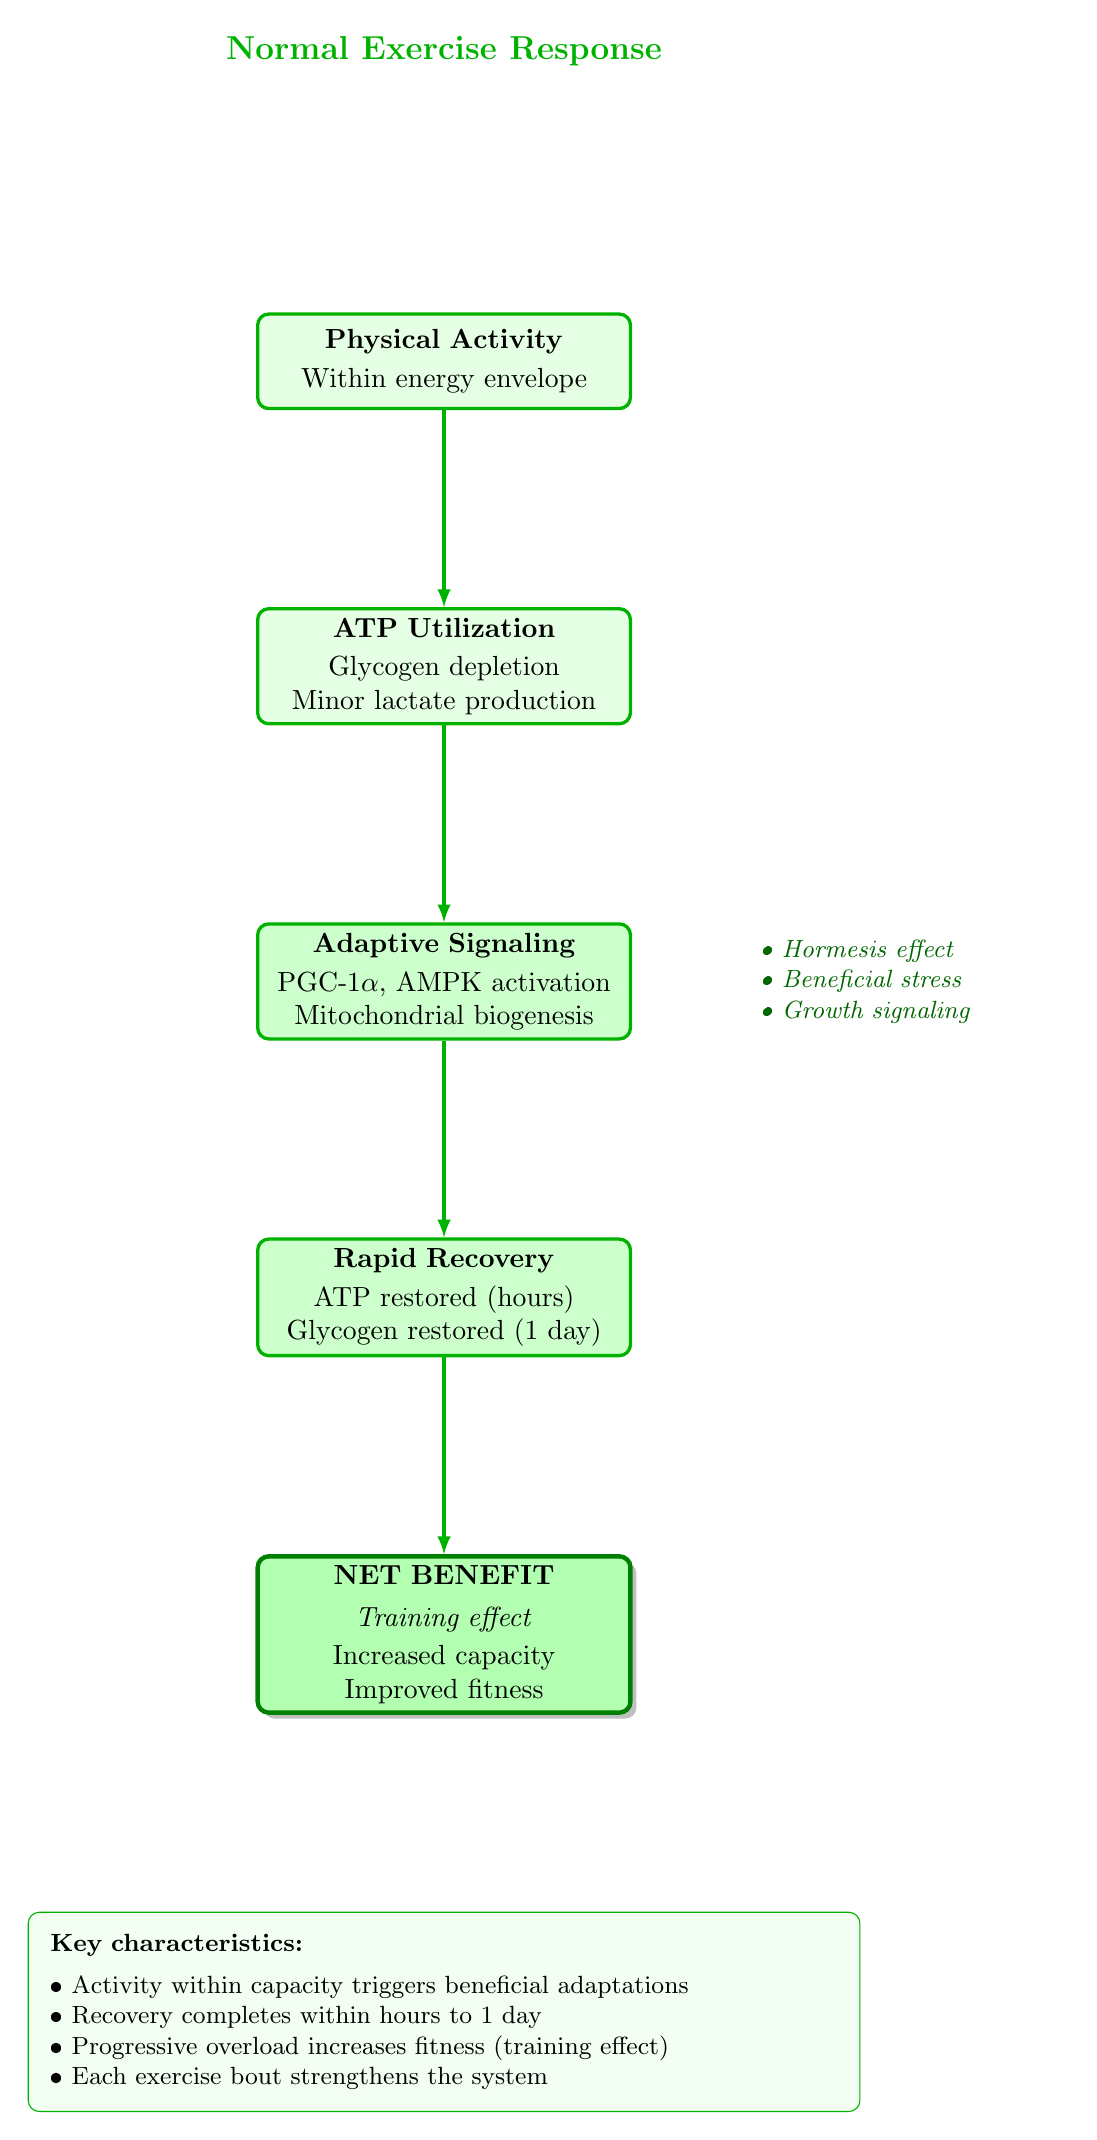
\begin{tikzpicture}[
    node distance=2.5cm,  % Global minimum vertical spacing
    % Styles
    process/.style={draw=green!70!black, fill=green!10, very thick, rounded corners, text width=4.5cm, align=center, minimum height=1.2cm},
    adaptive/.style={draw=green!70!black, fill=green!20, very thick, rounded corners, text width=4.5cm, align=center, minimum height=1.2cm},
    benefit/.style={draw=green!50!black, fill=green!30, ultra thick, rounded corners, text width=4.5cm, align=center, minimum height=1.3cm, drop shadow},
    arrow/.style={-latex, very thick, green!70!black, line width=1.2pt},
    note/.style={font=\small\itshape, text width=3.8cm, align=left, green!40!black},
]

% Title (absolute positioning OK for titles)
\node[font=\large\bfseries, green!70!black] (title) at (0, 0) {Normal Exercise Response};

% Exercise - first node, positioned relative to title
\node[process, below=3cm of title] (exercise) {\textbf{Physical Activity}\\[2pt] Within energy envelope};

% Metabolic response - relative positioning with minimum spacing
\node[process, below=of exercise] (atp) {\textbf{ATP Utilization}\\[2pt] Glycogen depletion\\Minor lactate production};
\draw[arrow] (exercise) -- (atp);

% Adaptive signaling
\node[adaptive, below=of atp] (signaling) {\textbf{Adaptive Signaling}\\[2pt] PGC-1$\alpha$, AMPK activation\\Mitochondrial biogenesis};
\draw[arrow] (atp) -- (signaling);

% Note positioned to the right
\node[note, right=1.5cm of signaling, anchor=west] {
    \textbullet~Hormesis effect\\
    \textbullet~Beneficial stress\\
    \textbullet~Growth signaling
};

% Recovery
\node[adaptive, below=of signaling] (recovery) {\textbf{Rapid Recovery}\\[2pt] ATP restored (hours)\\Glycogen restored (1 day)};
\draw[arrow] (signaling) -- (recovery);

% Positive outcome
\node[benefit, below=of recovery] (outcome) {\textbf{NET BENEFIT}\\[3pt] \textit{Training effect}\\[2pt] Increased capacity\\Improved fitness};
\draw[arrow] (recovery) -- (outcome);

% Key point box - positioned relative to outcome
\node[draw=green!70!black, fill=green!5, rounded corners, text width=10cm, align=left, font=\small, inner sep=8pt, below=2.5cm of outcome] {
\textbf{Key characteristics:}\\[4pt]
\textbullet~Activity within capacity triggers beneficial adaptations\\
\textbullet~Recovery completes within hours to 1 day\\
\textbullet~Progressive overload increases fitness (training effect)\\
\textbullet~Each exercise bout strengthens the system
};

\end{tikzpicture}
\caption{Normal exercise response with adaptive signaling and rapid recovery.}
\label{fig:pem-normal}
\end{figure}
\clearpage
% Figure: Post-Exertional Malaise (PEM) in ME/CFS
% Activity triggers harmful cascade with delayed worsening

\begin{figure}[htbp]
\centering
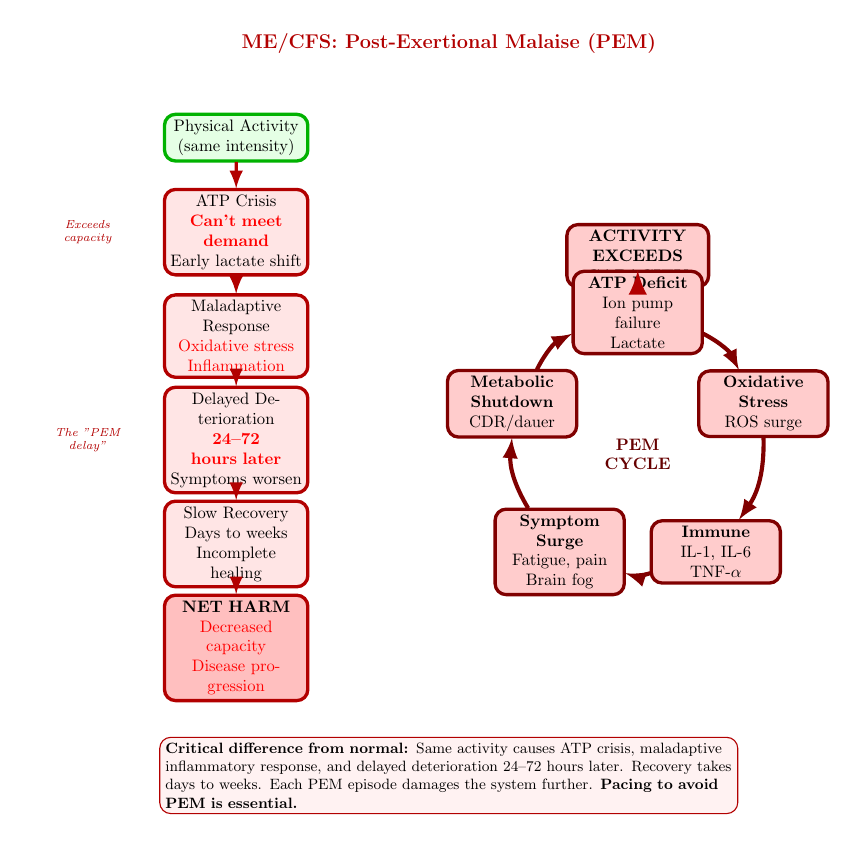
\begin{tikzpicture}[scale=0.60, every node/.style={scale=0.60},
    % Styles
    normal/.style={draw=green!70!black, fill=green!10, very thick, rounded corners, text width=2.8cm, align=center, minimum height=0.9cm},
    impaired/.style={draw=red!70!black, fill=red!10, very thick, rounded corners, text width=2.8cm, align=center, minimum height=0.9cm},
    pathological/.style={draw=red!50!black, fill=red!20, very thick, rounded corners, text width=2.5cm, align=center, minimum height=0.9cm},
    impaired-arrow/.style={-latex, very thick, red!70!black},
    cycle-arrow/.style={-latex, ultra thick, red!50!black, line width=1.5pt},
    note/.style={font=\scriptsize\itshape, text width=2.3cm, align=center},
]

% Title
\node[font=\large\bfseries, red!70!black] at (0, 9.5) {ME/CFS: Post-Exertional Malaise (PEM)};

% LEFT SIDE: Maladaptive response
\begin{scope}[xshift=-4.5cm]
    % Activity
    \node[normal] (exercise) at (0, 7.5) {Physical Activity\\(same intensity)};

    % ATP crisis
    \node[impaired] (atp) at (0, 5.5) {ATP Crisis\\{\color{red}\textbf{Can't meet demand}}\\Early lactate shift};
    \draw[impaired-arrow] (exercise) -- (atp);
    \node[note, left=0.2cm of atp, text=red!70!black] {Exceeds\\capacity};

    % Maladaptive response
    \node[impaired] (maladaptive) at (0, 3.3) {Maladaptive Response\\{\color{red}Oxidative stress}\\{\color{red}Inflammation}};
    \draw[impaired-arrow] (atp) -- (maladaptive);

    % Delayed crash
    \node[impaired] (delayed) at (0, 1.1) {Delayed Deterioration\\{\color{red}\textbf{24--72 hours later}}\\Symptoms worsen};
    \draw[impaired-arrow] (maladaptive) -- (delayed);
    \node[note, left=0.2cm of delayed, text=red!70!black] {The "PEM\\delay"};

    % Poor recovery
    \node[impaired] (poor) at (0, -1.1) {Slow Recovery\\Days to weeks\\Incomplete healing};
    \draw[impaired-arrow] (delayed) -- (poor);

    % Negative outcome
    \node[impaired, fill=red!25] (outcome) at (0, -3.3) {\textbf{NET HARM}\\{\color{red}Decreased capacity}\\{\color{red}Disease progression}};
    \draw[impaired-arrow] (poor) -- (outcome);
\end{scope}

% RIGHT SIDE: PEM vicious cycle
\begin{scope}[xshift=4cm, yshift=1cm]
    \def\radius{2.8}
    \def\centerx{0}
    \def\centery{0}

    % Trigger
    \node[pathological, minimum width=3cm] (trigger) at (\centerx, \centery + \radius + 1.2)
        {\textbf{ACTIVITY}\\  \textbf{EXCEEDS CAPACITY}};

    % Node 1: ATP deficit
    \node[pathological] (atp-def) at (\centerx, \centery + \radius)
        {\textbf{ATP Deficit}\\Ion pump failure\\Lactate};

    % Node 2: Oxidative stress
    \node[pathological] (ox) at (\centerx + \radius*0.95, \centery + \radius*0.31)
        {\textbf{Oxidative}\\  \textbf{Stress}\\ROS surge};

    % Node 3: Immune activation
    \node[pathological] (immune) at (\centerx + \radius*0.59, \centery - \radius*0.81)
        {\textbf{Immune}\\IL-1, IL-6\\TNF-$\alpha$};

    % Node 4: Symptoms
    \node[pathological] (symptoms) at (\centerx - \radius*0.59, \centery - \radius*0.81)
        {\textbf{Symptom}\\  \textbf{Surge}\\Fatigue, pain\\Brain fog};

    % Node 5: Metabolic suppression
    \node[pathological] (metabolic) at (\centerx - \radius*0.95, \centery + \radius*0.31)
        {\textbf{Metabolic}\\  \textbf{Shutdown}\\CDR/dauer};

    % Arrow from trigger
    \draw[impaired-arrow, line width=2pt] (trigger) -- (atp-def);

    % Cycle arrows
    \draw[cycle-arrow, bend left=18] (atp-def) to (ox);
    \draw[cycle-arrow, bend left=18] (ox) to (immune);
    \draw[cycle-arrow, bend left=18] (immune) to (symptoms);
    \draw[cycle-arrow, bend left=18] (symptoms) to (metabolic);
    \draw[cycle-arrow, bend left=18] (metabolic) to (atp-def);

    % Central label
    \node[font=\bfseries, red!40!black] at (\centerx, \centery) {PEM};
    \node[font=\bfseries, red!40!black] at (\centerx, \centery - 0.4) {CYCLE};
\end{scope}

% Key point box
\node[draw=red!70!black, fill=red!5, rounded corners, text width=12cm, align=left, font=\small] at (0, -6) {
\textbf{Critical difference from normal:} Same activity causes ATP crisis, maladaptive inflammatory response, and delayed deterioration 24--72 hours later. Recovery takes days to weeks. Each PEM episode damages the system further. \textbf{Pacing to avoid PEM is essential.}
};

\end{tikzpicture}
\caption{ME/CFS post-exertional malaise mechanism with harmful vicious cycle.}
\label{fig:pem-mecfs}
\end{figure}

\clearpage

% Energy
% Figure: Normal Cellular Energy Production
% How healthy cells produce ATP through glycolysis, Krebs cycle, and oxidative phosphorylation

\begin{figure}[htbp]
\centering
\begin{tikzpicture}[scale=0.75, every node/.style={scale=0.75},
    % Styles
    process/.style={draw=green!70!black, fill=green!10, very thick, rounded corners, text width=4cm, align=center, minimum height=1.2cm},
    output/.style={draw=green!70!black, fill=green!25, very thick, rounded corners, text width=4cm, align=center, minimum height=1.2cm},
    arrow/.style={-latex, very thick, green!70!black},
    note/.style={font=\small\itshape, text width=3.5cm, align=center},
]

% Title
\node[font=\large\bfseries, green!70!black] at (0, 9) {Normal Cellular Energy Production};

% Glucose input
\node[process] (glucose) at (0, 7.5) {\textbf{Glucose}\\(from food digestion)};

% Glycolysis
\node[process] (glycolysis) at (0, 5.5) {\textbf{Glycolysis}\\(in cytosol)};
\draw[arrow] (glucose) -- (glycolysis);
\node[note, right=1cm of glycolysis] {Produces:\\2 ATP\\2 NADH\\2 Pyruvate};

% Pyruvate conversion
\node[process] (pyruvate) at (0, 3.5) {\textbf{Pyruvate $\rightarrow$ Acetyl-CoA}\\(enters mitochondria)};
\draw[arrow] (glycolysis) -- (pyruvate);

% Krebs Cycle
\node[process] (krebs) at (0, 1.5) {\textbf{Krebs Cycle}\\(mitochondrial matrix)};
\draw[arrow] (pyruvate) -- (krebs);
\node[note, right=1cm of krebs] {Produces:\\3 NADH, FADH\textsubscript{2}\\GTP per cycle};

% Electron Transport Chain
\node[process] (etc) at (0, -0.5) {\textbf{Electron Transport Chain}\\(Complexes I--IV)};
\draw[arrow] (krebs) -- (etc);
\node[note, right=1cm of etc] {Electron leak:\\$<$2\% normal};

% ATP output
\node[output] (atp) at (0, -2.7) {\textbf{30--32 ATP per glucose}\\Abundant cellular energy};
\draw[arrow] (etc) -- (atp);

% Key point box
\node[draw=green!70!black, fill=green!5, rounded corners, text width=10cm, align=left, font=\small] at (0, -5) {
\textbf{Key points:}
\begin{itemize}[leftmargin=*, nosep, topsep=2pt]
\item Efficient conversion of glucose to ATP
\item Minimal electron leakage ($<$2\%) in healthy mitochondria
\item NADH and FADH\textsubscript{2} carry electrons to the ETC
\item Brain uses 20\% of total ATP production at rest
\end{itemize}
};

\end{tikzpicture}
\caption{Normal cellular energy production pathway.}
\label{fig:energy-cascade-normal}
\end{figure}

\clearpage
% Figure: Impaired Energy Production in ME/CFS
% Multiple dysfunction points reduce ATP and cause system-wide failures

\begin{figure}[htbp]
\centering
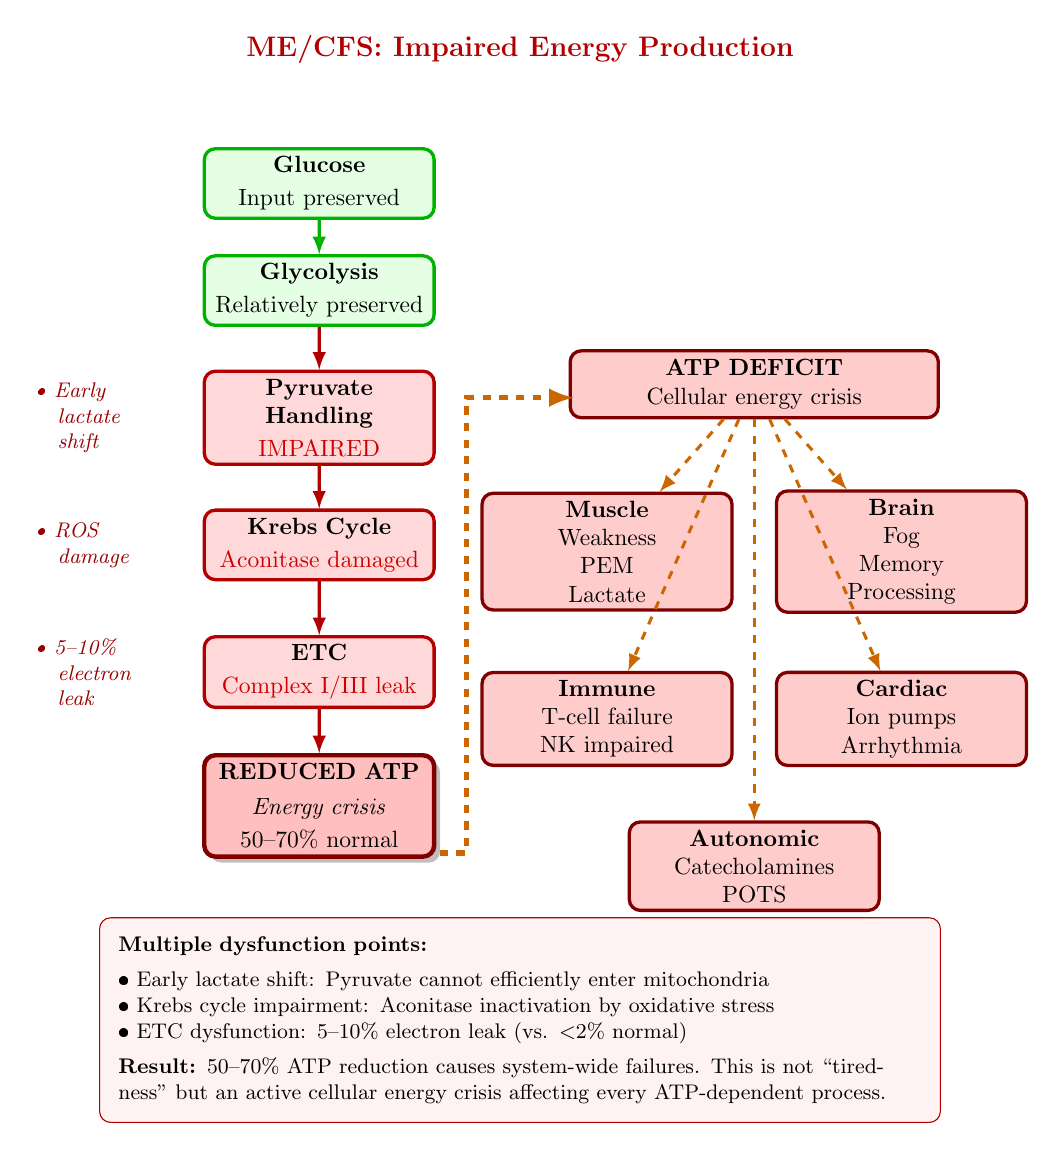
\begin{tikzpicture}[
    node distance=2.5cm,
    scale=0.85, every node/.style={scale=0.85},
    % Styles
    normal/.style={draw=green!70!black, fill=green!10, very thick, rounded corners, text width=3.2cm, align=center, minimum height=1cm},
    impaired/.style={draw=red!70!black, fill=red!15, very thick, rounded corners, text width=3.2cm, align=center, minimum height=1cm},
    severe/.style={draw=red!50!black, fill=red!25, ultra thick, rounded corners, text width=3.2cm, align=center, minimum height=1.1cm, drop shadow},
    pathological/.style={draw=red!50!black, fill=red!20, very thick, rounded corners, text width=3.5cm, align=center, minimum height=1cm},
    arrow/.style={-latex, very thick, green!70!black, line width=1.2pt},
    impaired-arrow/.style={-latex, very thick, red!70!black, line width=1.2pt},
    cascade-arrow/.style={-latex, thick, orange!80!black, dashed, line width=1.1pt},
    note/.style={font=\small\itshape, text width=2.2cm, align=left, red!60!black},
]

% Title
\node[font=\large\bfseries, red!70!black] at (0, 9) {ME/CFS: Impaired Energy Production};

% LEFT SIDE: Impaired pathway
\begin{scope}[xshift=-3cm]
    % Glucose (preserved)
    \node[normal] (glucose) at (0, 7) {\textbf{Glucose}\\[2pt] Input preserved};

    % Glycolysis (relatively preserved)
    \node[normal] (glycolysis) at (0, 5.4) {\textbf{Glycolysis}\\[2pt] Relatively preserved};
    \draw[arrow] (glucose) -- (glycolysis);

    % Pyruvate - IMPAIRED
    \node[impaired] (pyruvate) at (0, 3.5) {\textbf{Pyruvate Handling}\\[2pt] {\color{red!80!black}IMPAIRED}};
    \draw[impaired-arrow] (glycolysis) -- (pyruvate);
    \node[note, left=0.15cm of pyruvate, anchor=east] {
        \textbullet~Early\\~~~lactate\\~~~shift
    };

    % Krebs - IMPAIRED
    \node[impaired] (krebs) at (0, 1.6) {\textbf{Krebs Cycle}\\[2pt] {\color{red!80!black}Aconitase damaged}};
    \draw[impaired-arrow] (pyruvate) -- (krebs);
    \node[note, left=0.15cm of krebs, anchor=east] {
        \textbullet~ROS\\~~~damage
    };

    % ETC - IMPAIRED
    \node[impaired] (etc) at (0, -0.3) {\textbf{ETC}\\[2pt] {\color{red!80!black}Complex I/III leak}};
    \draw[impaired-arrow] (krebs) -- (etc);
    \node[note, left=0.15cm of etc, anchor=east] {
        \textbullet~5--10\%\\~~~electron\\~~~leak
    };

    % ATP - REDUCED
    \node[severe] (atp) at (0, -2.3) {\textbf{REDUCED ATP}\\[3pt] \textit{Energy crisis}\\[2pt] 50--70\% normal};
    \draw[impaired-arrow] (etc) -- (atp);
\end{scope}

% RIGHT SIDE: System failures from ATP deficit
\begin{scope}[xshift=3.5cm]
    % Central deficit node
    \node[pathological, minimum width=5.5cm, text width=4cm,] (deficit) at (0, 4) {\textbf{ATP DEFICIT}\\Cellular energy crisis};

    % System failures
    \node[pathological] (muscle) at (-2.2, 1.5) {\textbf{Muscle}\\Weakness\\PEM\\Lactate};

    \node[pathological] (brain) at (2.2, 1.5) {\textbf{Brain}\\Fog\\Memory\\Processing};

    \node[pathological] (immune) at (-2.2, -1) {\textbf{Immune}\\T-cell failure\\NK impaired};

    \node[pathological] (cardio) at (2.2, -1) {\textbf{Cardiac}\\Ion pumps\\Arrhythmia};

    \node[pathological] (autonomic) at (0, -3.2) {\textbf{Autonomic}\\Catecholamines\\POTS};

    % Cascade arrows
    \draw[cascade-arrow] (deficit) -- (muscle);
    \draw[cascade-arrow] (deficit) -- (brain);
    \draw[cascade-arrow] (deficit) -- (immune);
    \draw[cascade-arrow] (deficit) -- (cardio);
    \draw[cascade-arrow] (deficit) -- (autonomic);
\end{scope}

% Arrow connecting left to right
\draw[cascade-arrow, line width=2pt] (-1.2, -3) -- (-0.8, -3) -- (-0.8, 3.8) -- (0.8, 3.8);

% Key point box
\node[draw=red!70!black, fill=red!5, rounded corners, text width=12cm, align=left, font=\small, inner sep=8pt] at (0, -5.5) {
\textbf{Multiple dysfunction points:}\\[4pt]
\textbullet~Early lactate shift: Pyruvate cannot efficiently enter mitochondria\\
\textbullet~Krebs cycle impairment: Aconitase inactivation by oxidative stress\\
\textbullet~ETC dysfunction: 5--10\% electron leak (vs. $<$2\% normal)\\[4pt]
\textbf{Result:} 50--70\% ATP reduction causes system-wide failures. This is not ``tiredness'' but an active cellular energy crisis affecting every ATP-dependent process.
};

\end{tikzpicture}
\caption{ME/CFS energy production dysfunction and systemic consequences.}
\label{fig:energy-cascade-mecfs}
\end{figure}

\clearpage

% Oxidative Stress
% Figure: Normal Oxidative Stress Balance
% Healthy balance between ROS production and antioxidant defense

\begin{figure}[htbp]
\centering
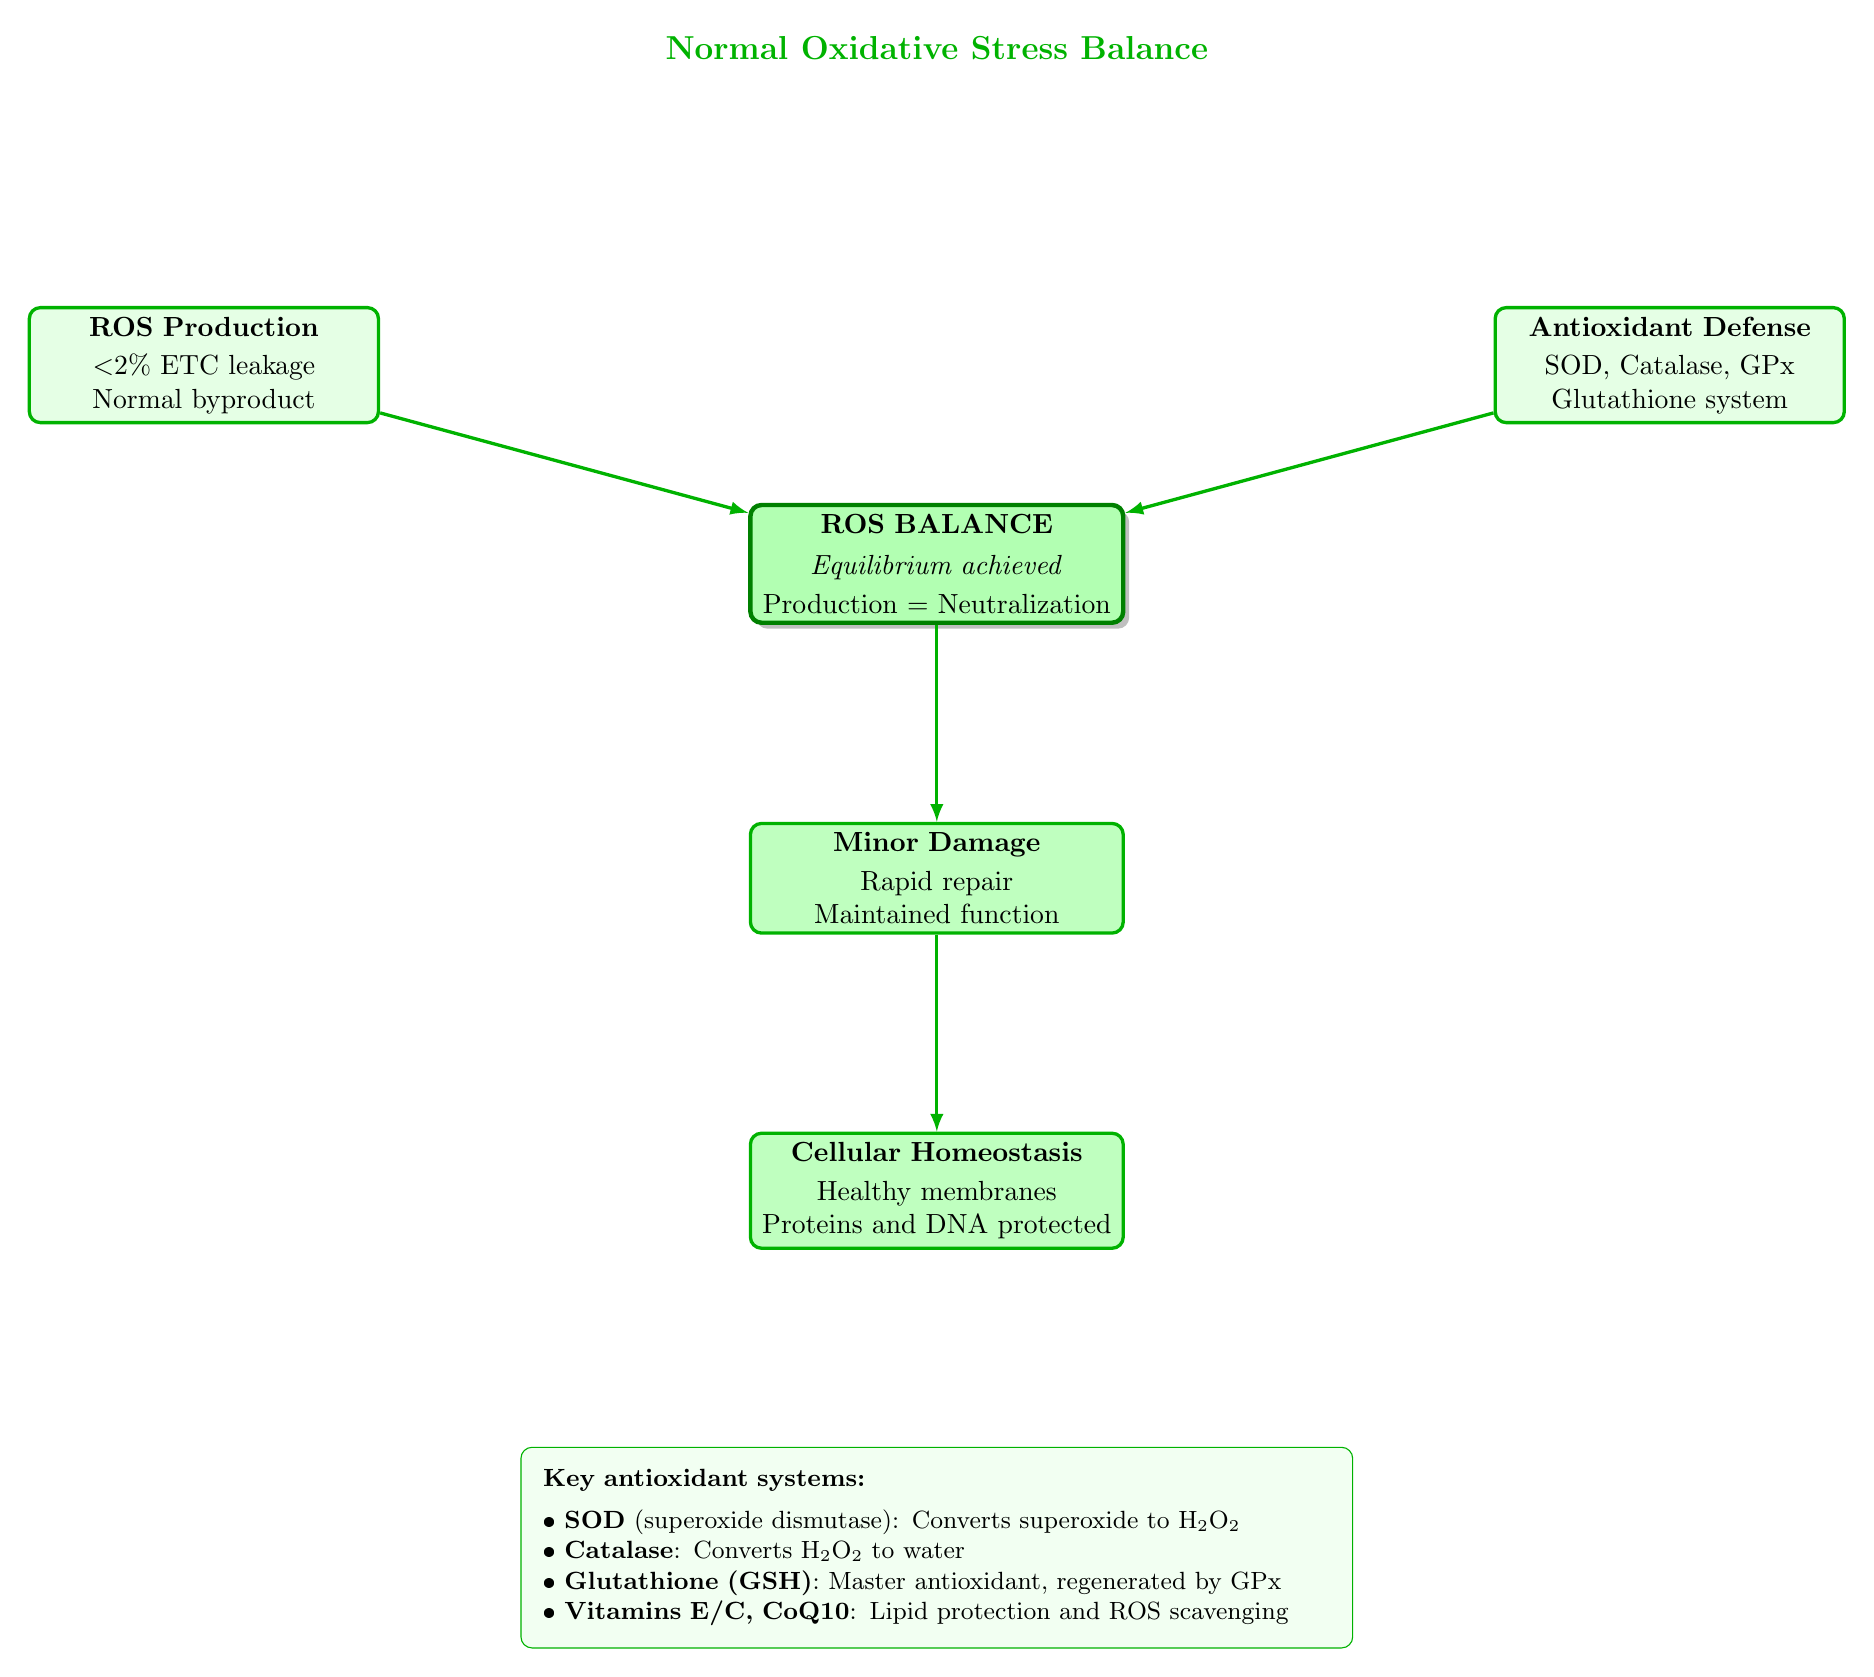
\begin{tikzpicture}[
    node distance=2.5cm,  % Global minimum vertical spacing
    % Styles
    process/.style={draw=green!70!black, fill=green!10, very thick, rounded corners, text width=4.2cm, align=center, minimum height=1.2cm},
    balanced/.style={draw=green!50!black, fill=green!30, ultra thick, rounded corners, text width=4.5cm, align=center, minimum height=1.3cm, drop shadow},
    output/.style={draw=green!70!black, fill=green!25, very thick, rounded corners, text width=4.5cm, align=center, minimum height=1.2cm},
    arrow/.style={-latex, very thick, green!70!black, line width=1.2pt},
    note/.style={font=\small\itshape, text width=3.5cm, align=left, green!40!black},
]

% Title
\node[font=\large\bfseries, green!70!black] (title) at (0, 0) {Normal Oxidative Stress Balance};

% ROS production (left)
\node[process, below left=3cm and 3.5cm of title] (ros) {\textbf{ROS Production}\\[2pt] $<$2\% ETC leakage\\Normal byproduct};

% Antioxidant defense (right)
\node[process, below right=3cm and 3.5cm of title] (antioxidants) {\textbf{Antioxidant Defense}\\[2pt] SOD, Catalase, GPx\\Glutathione system};

% Balance point
\node[balanced, below=5.5cm of title] (balance) {\textbf{ROS BALANCE}\\[3pt] \textit{Equilibrium achieved}\\[2pt] Production = Neutralization};

\draw[arrow] (ros) -- (balance);
\draw[arrow] (antioxidants) -- (balance);

% Minor damage and repair
\node[output, below=of balance] (repair) {\textbf{Minor Damage}\\[2pt] Rapid repair\\Maintained function};
\draw[arrow] (balance) -- (repair);

% Outcome
\node[output, below=of repair] (outcome) {\textbf{Cellular Homeostasis}\\[2pt] Healthy membranes\\Proteins and DNA protected};
\draw[arrow] (repair) -- (outcome);

% Key point box
\node[draw=green!70!black, fill=green!5, rounded corners, text width=10cm, align=left, font=\small, inner sep=8pt, below=2.5cm of outcome] {
\textbf{Key antioxidant systems:}\\[4pt]
\textbullet~\textbf{SOD} (superoxide dismutase): Converts superoxide to H$_2$O$_2$\\
\textbullet~\textbf{Catalase}: Converts H$_2$O$_2$ to water\\
\textbullet~\textbf{Glutathione (GSH)}: Master antioxidant, regenerated by GPx\\
\textbullet~\textbf{Vitamins E/C, CoQ10}: Lipid protection and ROS scavenging
};

\end{tikzpicture}
\caption{Normal oxidative stress homeostasis with balanced ROS production and neutralization.}
\label{fig:oxidative-stress-normal}
\end{figure}

\clearpage
% Figure: Oxidative Stress Vicious Cycle in ME/CFS
% Imbalance creates self-perpetuating damage cascade

\begin{figure}[htbp]
\centering
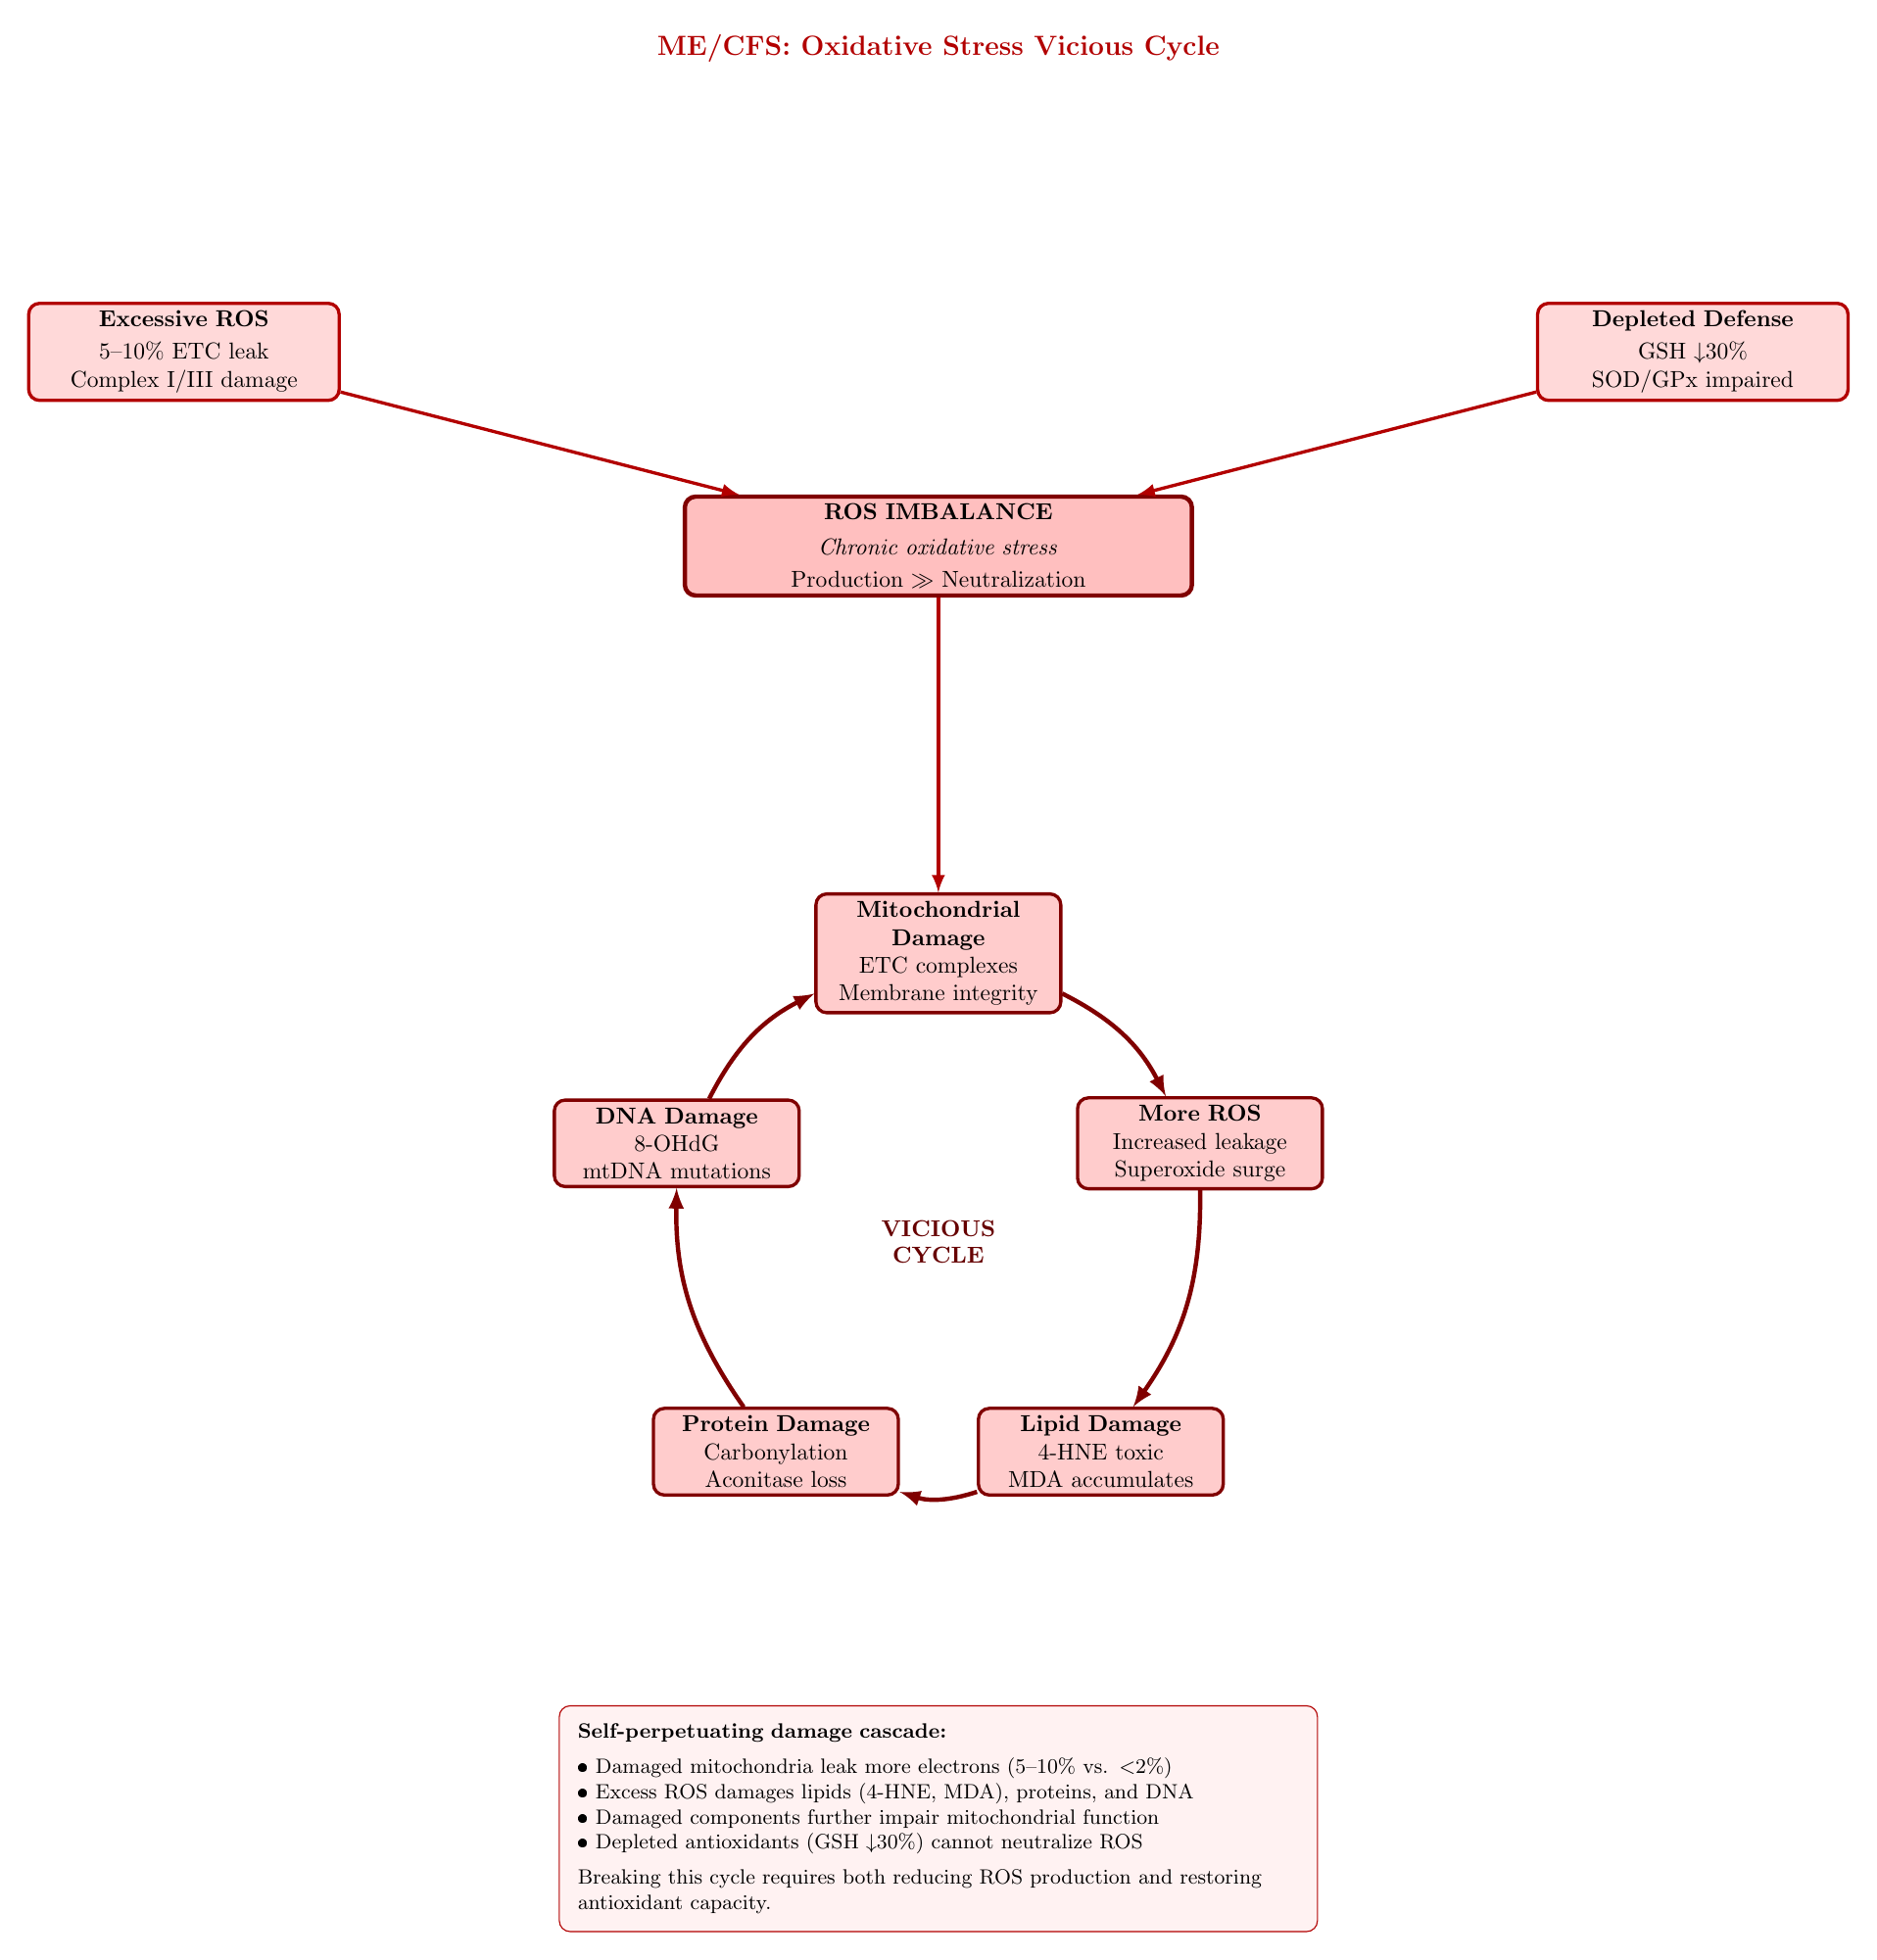
\begin{tikzpicture}[
    node distance=2.5cm,  % Global minimum vertical spacing
    scale=0.85, every node/.style={scale=0.85},
    % Styles
    impaired/.style={draw=red!70!black, fill=red!15, very thick, rounded corners, text width=4.5cm, align=center, minimum height=1cm},
    severe/.style={draw=red!50!black, fill=red!25, ultra thick, rounded corners, text width=7.5cm, align=center, minimum height=1.1cm},
    pathological/.style={draw=red!50!black, fill=red!20, very thick, rounded corners, text width=3.5cm, align=center, minimum height=1cm},
    impaired-arrow/.style={-latex, very thick, red!70!black, line width=1.2pt},
    cycle-arrow/.style={-latex, ultra thick, red!50!black, line width=1.6pt},
    note/.style={font=\small\itshape, text width=2.5cm, align=left, red!60!black},
]

% Title
\node[font=\large\bfseries, red!70!black] (title) at (0, 0) {ME/CFS: Oxidative Stress Vicious Cycle};

% TOP: Imbalance
\begin{scope}[yshift=-3cm]
    % Excessive ROS (left)
    \node[impaired, below left=3cm and 4cm of title] (ros) {\textbf{Excessive ROS}\\[2pt] 5--10\% ETC leak\\Complex I/III damage};

    % Depleted antioxidants (right)
    \node[impaired, below right=3cm and 4cm of title] (antioxidants) {\textbf{Depleted Defense}\\[2pt] GSH $\downarrow$30\%\\SOD/GPx impaired};

    % Imbalance
    \node[severe, below=5.5cm of title] (imbalance) {\textbf{ROS IMBALANCE}\\[3pt] \textit{Chronic oxidative stress}\\[2pt] Production $\gg$ Neutralization};

    \draw[impaired-arrow] (ros) -- (imbalance);
    \draw[impaired-arrow] (antioxidants) -- (imbalance);
\end{scope}

% BOTTOM: Vicious cycle with proper radius
\begin{scope}[yshift=-18cm]
    \def\radius{4.2}  % Increased from 4.0cm for better spacing
    \def\centerx{0}
    \def\centery{0}

    % Node 1: Mitochondrial damage (top)
    \node[pathological] (mito) at (\centerx, \centery + \radius)
        {\textbf{Mitochondrial Damage}\\ETC complexes\\Membrane integrity};

    % Node 2: Increased ROS (right)
    \node[pathological] (ros-up) at (\centerx + \radius*0.95, \centery + \radius*0.31)
        {\textbf{More ROS}\\Increased leakage\\Superoxide surge};

    % Node 3: Lipid peroxidation (bottom right)
    \node[pathological] (lipid) at (\centerx + \radius*0.59, \centery - \radius*0.81)
        {\textbf{Lipid Damage}\\4-HNE toxic\\MDA accumulates};

    % Node 4: Protein damage (bottom left)
    \node[pathological] (protein) at (\centerx - \radius*0.59, \centery - \radius*0.81)
        {\textbf{Protein Damage}\\Carbonylation\\Aconitase loss};

    % Node 5: DNA damage (left)
    \node[pathological] (dna) at (\centerx - \radius*0.95, \centery + \radius*0.31)
        {\textbf{DNA Damage}\\8-OHdG\\mtDNA mutations};

    % Cycle arrows (clockwise)
    \draw[cycle-arrow, bend left=18] (mito) to (ros-up);
    \draw[cycle-arrow, bend left=18] (ros-up) to (lipid);
    \draw[cycle-arrow, bend left=18] (lipid) to (protein);
    \draw[cycle-arrow, bend left=18] (protein) to (dna);
    \draw[cycle-arrow, bend left=18] (dna) to (mito);

    % Central label
    \node[font=\bfseries, red!40!black] at (\centerx, \centery) {VICIOUS};
    \node[font=\bfseries, red!40!black] at (\centerx, \centery - 0.4) {CYCLE};
\end{scope}

% Arrow from imbalance to cycle
\draw[impaired-arrow] (imbalance) -- (mito);

% Key point box
\node[draw=red!70!black, fill=red!5, rounded corners, text width=11cm, align=left, font=\small, inner sep=8pt] at (0, -27) {
\textbf{Self-perpetuating damage cascade:}\\[4pt]
\textbullet~Damaged mitochondria leak more electrons (5--10\% vs. $<$2\%)\\
\textbullet~Excess ROS damages lipids (4-HNE, MDA), proteins, and DNA\\
\textbullet~Damaged components further impair mitochondrial function\\
\textbullet~Depleted antioxidants (GSH $\downarrow$30\%) cannot neutralize ROS\\[4pt]
Breaking this cycle requires both reducing ROS production and restoring antioxidant capacity.
};

\end{tikzpicture}
\caption{ME/CFS oxidative stress vicious cycle with self-perpetuating damage.}
\label{fig:oxidative-stress-mecfs}
\end{figure}

\clearpage

% HPA Axis
% Figure: Normal HPA Axis Function
% Appropriate stress response with negative feedback control

\begin{figure}[htbp]
\centering
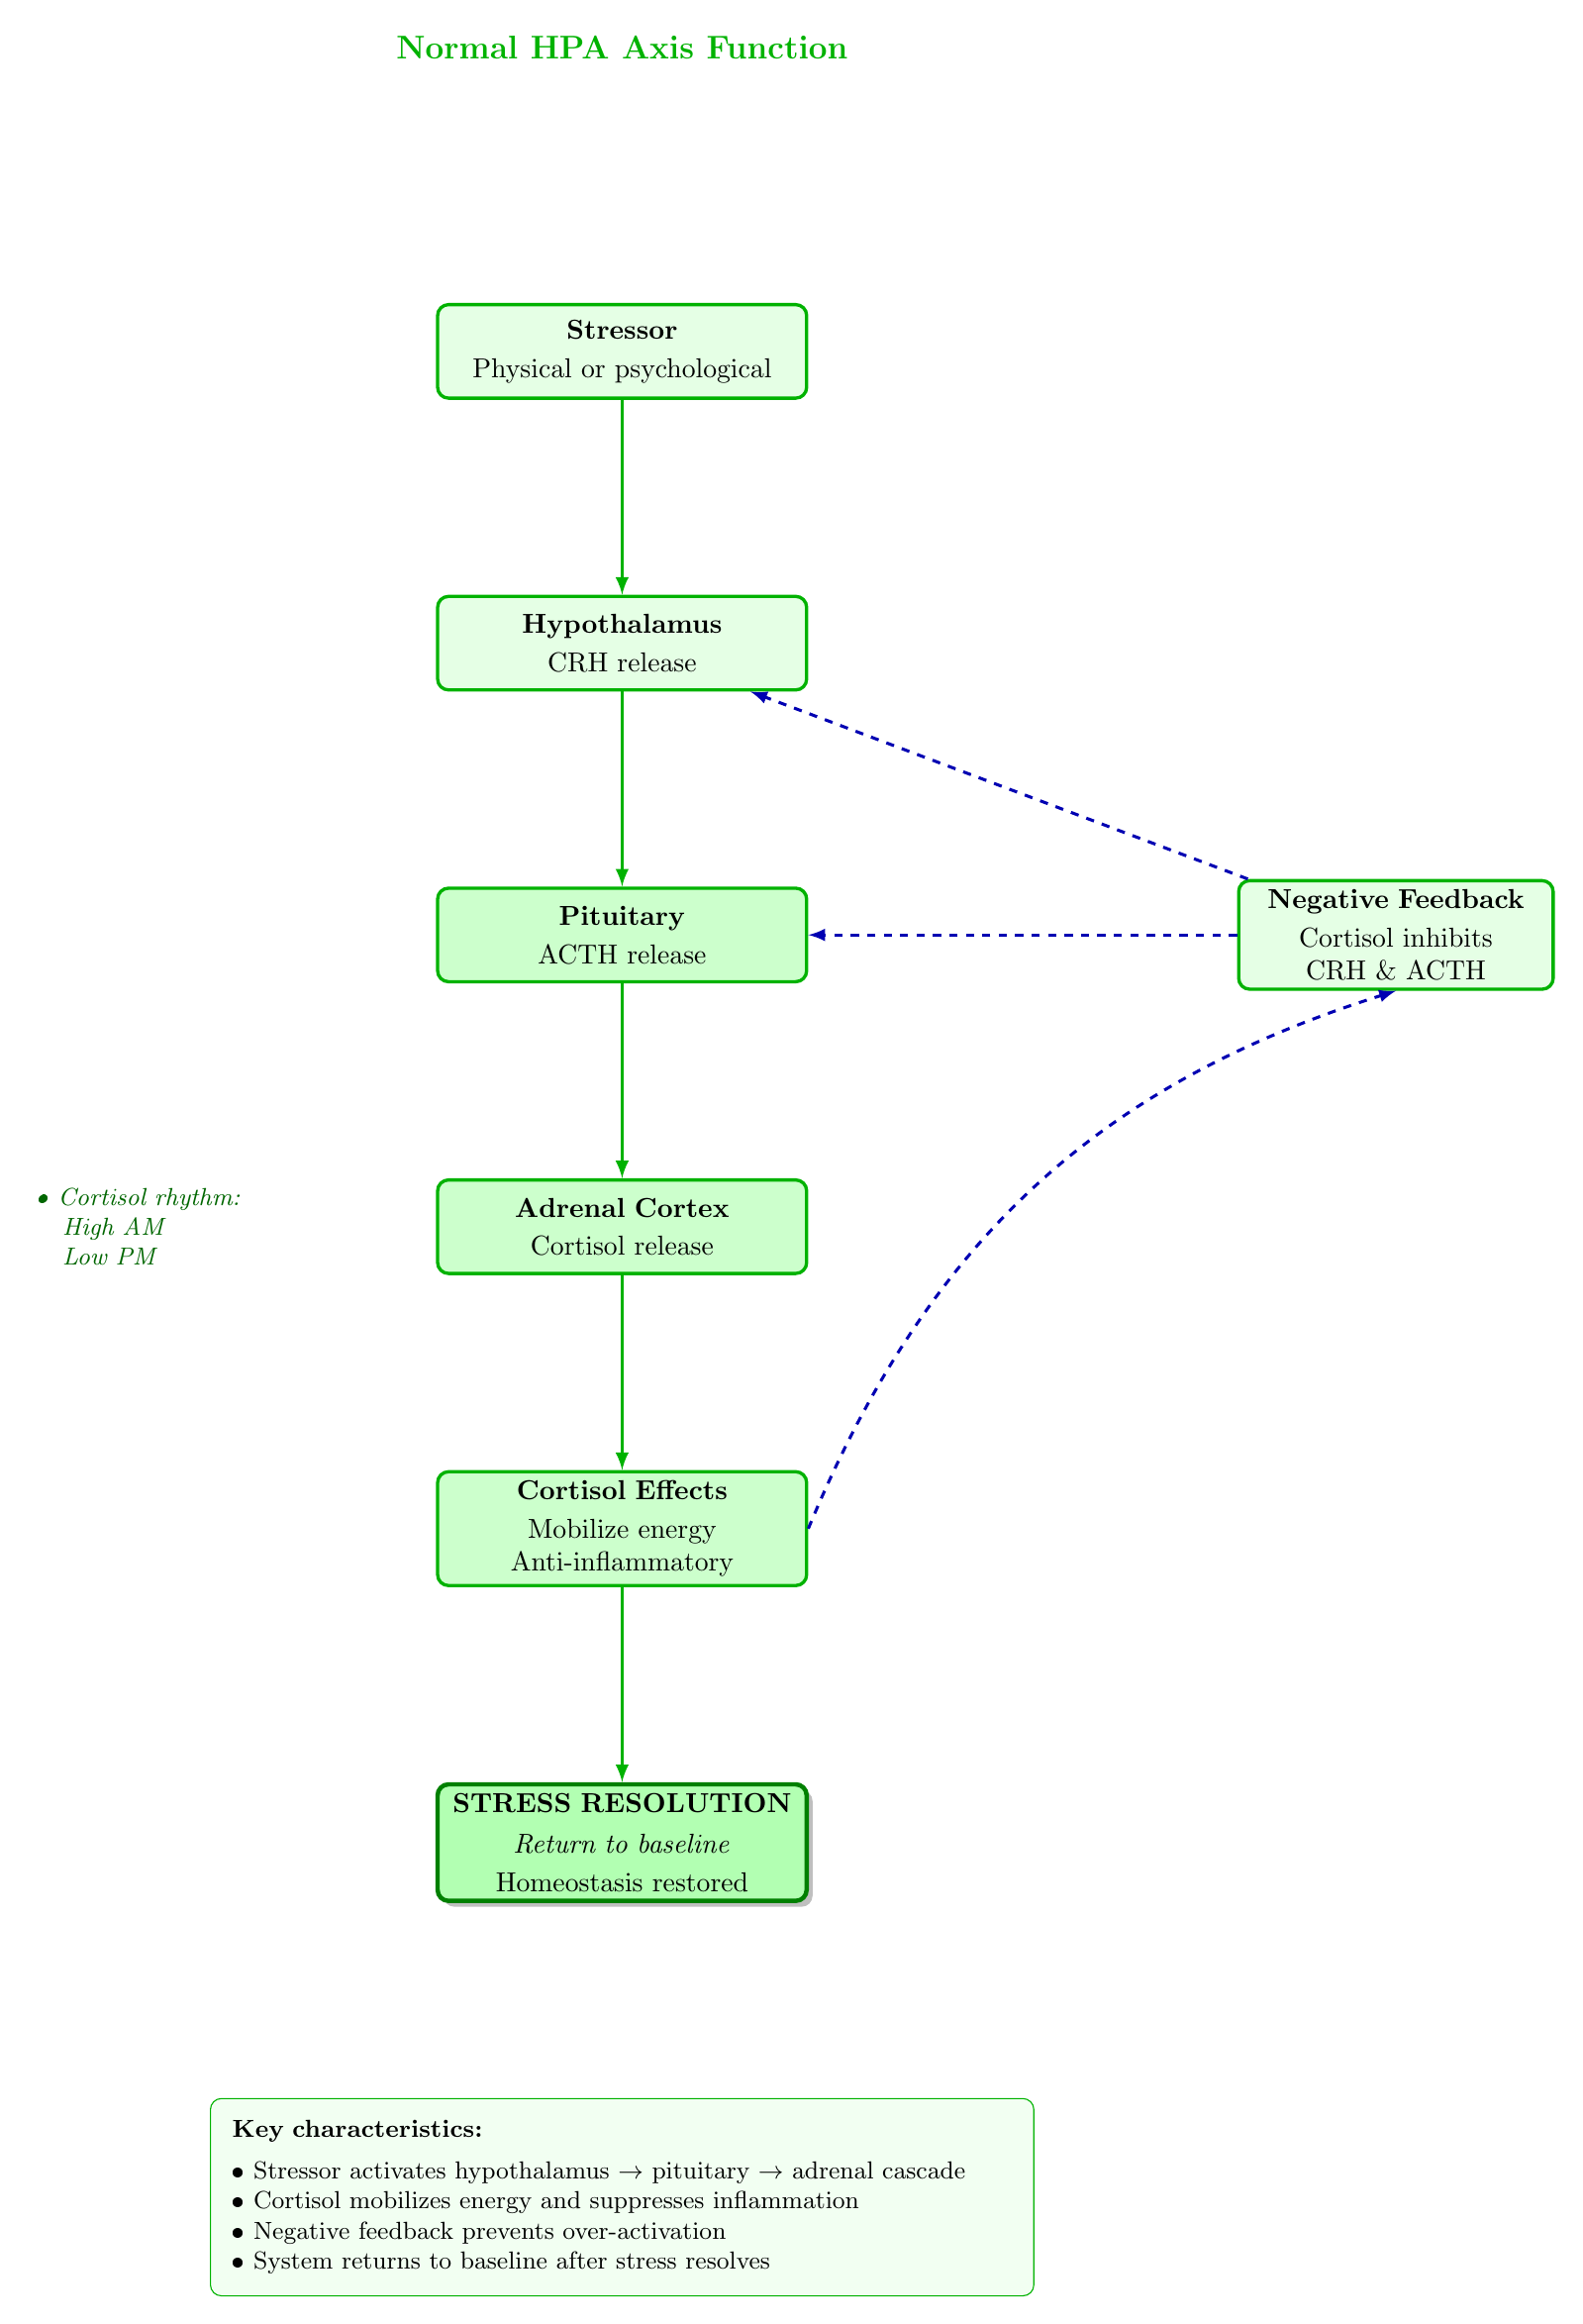
\begin{tikzpicture}[
    node distance=2.5cm,  % Global minimum vertical spacing
    % Styles
    process/.style={draw=green!70!black, fill=green!10, very thick, rounded corners, text width=4.5cm, align=center, minimum height=1.2cm},
    adaptive/.style={draw=green!70!black, fill=green!20, very thick, rounded corners, text width=4.5cm, align=center, minimum height=1.2cm},
    output/.style={draw=green!50!black, fill=green!30, ultra thick, rounded corners, text width=4.5cm, align=center, minimum height=1.3cm, drop shadow},
    arrow/.style={-latex, very thick, green!70!black, line width=1.2pt},
    feedback/.style={-latex, thick, blue!70!black, dashed, line width=1.1pt},
    note/.style={font=\small\itshape, text width=3.5cm, align=left, green!40!black},
]

% Title
\node[font=\large\bfseries, green!70!black] (title) at (0, 0) {Normal HPA Axis Function};

% Stressor
\node[process, below=3cm of title] (stressor) {\textbf{Stressor}\\[2pt] Physical or psychological};

% Hypothalamus
\node[process, below=of stressor] (hypothalamus) {\textbf{Hypothalamus}\\[2pt] CRH release};
\draw[arrow] (stressor) -- (hypothalamus);

% Pituitary
\node[adaptive, below=of hypothalamus] (pituitary) {\textbf{Pituitary}\\[2pt] ACTH release};
\draw[arrow] (hypothalamus) -- (pituitary);

% Adrenal
\node[adaptive, below=of pituitary] (adrenal) {\textbf{Adrenal Cortex}\\[2pt] Cortisol release};
\draw[arrow] (pituitary) -- (adrenal);
\node[note, left=1.5cm of adrenal, anchor=east] {
    \textbullet~Cortisol rhythm:\\~~~High AM\\~~~Low PM
};

% Cortisol effects
\node[adaptive, below=of adrenal] (cortisol) {\textbf{Cortisol Effects}\\[2pt] Mobilize energy\\Anti-inflammatory};
\draw[arrow] (adrenal) -- (cortisol);

% Negative feedback (right side)
\node[process, text width=3.8cm, right=5.5cm of pituitary] (feedback-box) {\textbf{Negative Feedback}\\[2pt] Cortisol inhibits\\CRH \& ACTH};
\draw[feedback, bend left=25] (cortisol.east) to (feedback-box.south);
\draw[feedback] (feedback-box) -- (hypothalamus);
\draw[feedback] (feedback-box) -- (pituitary);

% Recovery
\node[output, below=of cortisol] (recovery) {\textbf{STRESS RESOLUTION}\\[3pt] \textit{Return to baseline}\\[2pt] Homeostasis restored};
\draw[arrow] (cortisol) -- (recovery);

% Key point box
\node[draw=green!70!black, fill=green!5, rounded corners, text width=10cm, align=left, font=\small, inner sep=8pt, below=2.5cm of recovery] {
\textbf{Key characteristics:}\\[4pt]
\textbullet~Stressor activates hypothalamus $\rightarrow$ pituitary $\rightarrow$ adrenal cascade\\
\textbullet~Cortisol mobilizes energy and suppresses inflammation\\
\textbullet~Negative feedback prevents over-activation\\
\textbullet~System returns to baseline after stress resolves
};

\end{tikzpicture}
\caption{Normal HPA axis stress response with negative feedback control.}
\label{fig:hpa-axis-normal}
\end{figure}

\clearpage
% Figure: HPA Axis Dysregulation in ME/CFS
% Blunted response, excessive feedback, systemic consequences

\begin{figure}[htbp]
\centering
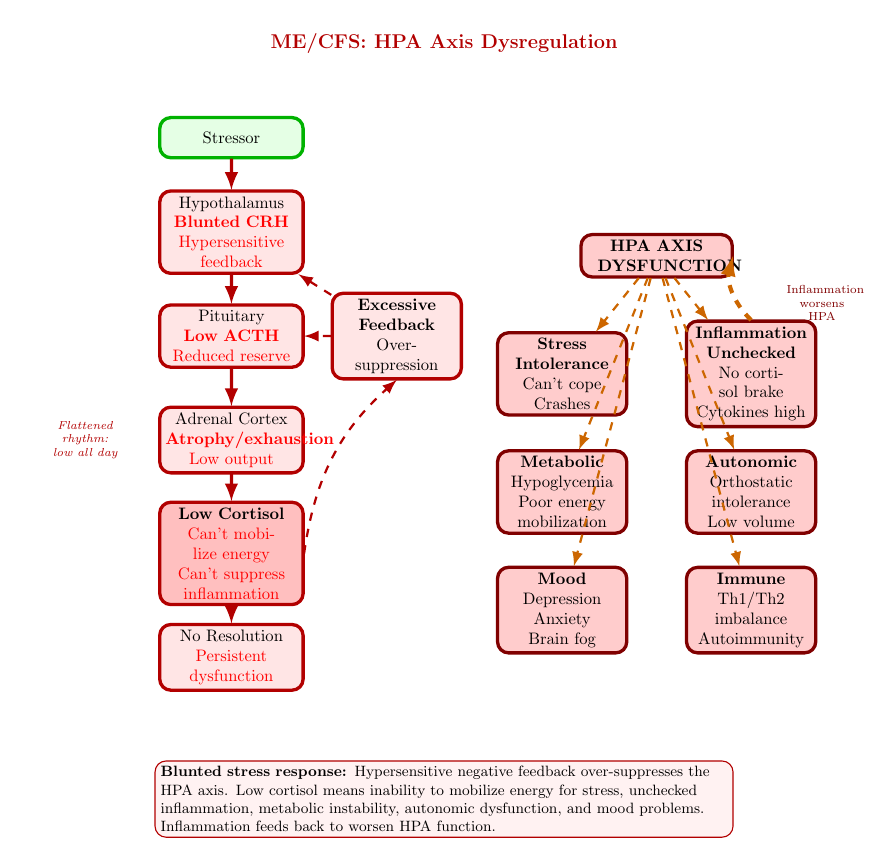
\begin{tikzpicture}[scale=0.60, every node/.style={scale=0.60},
    % Styles
    normal/.style={draw=green!70!black, fill=green!10, very thick, rounded corners, text width=2.8cm, align=center, minimum height=0.85cm},
    impaired/.style={draw=red!70!black, fill=red!10, very thick, rounded corners, text width=2.8cm, align=center, minimum height=0.85cm},
    pathological/.style={draw=red!50!black, fill=red!20, very thick, rounded corners, text width=2.5cm, align=center, minimum height=0.85cm},
    impaired-arrow/.style={-latex, very thick, red!70!black},
    feedback/.style={-latex, thick, red!70!black, dashed},
    cascade-arrow/.style={-latex, thick, orange!80!black, dashed},
    note/.style={font=\scriptsize\itshape, text width=2.2cm, align=center},
]

% Title
\node[font=\large\bfseries, red!70!black] at (0, 9.5) {ME/CFS: HPA Axis Dysregulation};

% LEFT SIDE: Impaired pathway
\begin{scope}[xshift=-4.5cm]
    % Stressor
    \node[normal] (stressor) at (0, 7.5) {Stressor};

    % Hypothalamus - blunted
    \node[impaired] (hypothalamus) at (0, 5.5) {Hypothalamus\\{\color{red}\textbf{Blunted CRH}}\\{\color{red}Hypersensitive feedback}};
    \draw[impaired-arrow] (stressor) -- (hypothalamus);

    % Pituitary - impaired
    \node[impaired] (pituitary) at (0, 3.3) {Pituitary\\{\color{red}\textbf{Low ACTH}}\\{\color{red}Reduced reserve}};
    \draw[impaired-arrow] (hypothalamus) -- (pituitary);

    % Adrenal - atrophy
    \node[impaired] (adrenal) at (0, 1.1) {Adrenal Cortex\\{\color{red}\textbf{Atrophy/exhaustion}}\\{\color{red}Low output}};
    \draw[impaired-arrow] (pituitary) -- (adrenal);
    \node[note, left=0.2cm of adrenal, text=red!70!black] {Flattened\\rhythm:\\low all day};

    % Low cortisol
    \node[impaired, fill=red!25] (cortisol) at (0, -1.3) {\textbf{Low Cortisol}\\{\color{red}Can't mobilize energy}\\{\color{red}Can't suppress inflammation}};
    \draw[impaired-arrow] (adrenal) -- (cortisol);

    % Excessive feedback
    \node[impaired, text width=2.5cm] (feedback-box) at (3.5, 3.3) {\textbf{Excessive}\\  \textbf{Feedback}\\Over-suppression};
    \draw[feedback, bend left=20] (cortisol.east) to (feedback-box.south);
    \draw[feedback] (feedback-box) -- (hypothalamus);
    \draw[feedback] (feedback-box) -- (pituitary);

    % No recovery
    \node[impaired] (no-recovery) at (0, -3.5) {No Resolution\\{\color{red}Persistent dysfunction}};
    \draw[impaired-arrow] (cortisol) -- (no-recovery);
\end{scope}

% RIGHT SIDE: System failures
\begin{scope}[xshift=4.5cm]
    % Central dysfunction
    \node[pathological, minimum width=3.2cm] (hpa) at (0, 5) {\textbf{HPA AXIS}\\  \textbf{DYSFUNCTION}};

    % Six consequences in 2x3 grid
    \node[pathological] (stress) at (-2, 2.5) {\textbf{Stress}\\  \textbf{Intolerance}\\Can't cope\\Crashes};

    \node[pathological] (inflam) at (2, 2.5) {\textbf{Inflammation}\\  \textbf{Unchecked}\\No cortisol brake\\Cytokines high};

    \node[pathological] (metabolic) at (-2, 0) {\textbf{Metabolic}\\Hypoglycemia\\Poor energy\\mobilization};

    \node[pathological] (autonomic) at (2, 0) {\textbf{Autonomic}\\Orthostatic\\intolerance\\Low volume};

    \node[pathological] (mood) at (-2, -2.5) {\textbf{Mood}\\Depression\\Anxiety\\Brain fog};

    \node[pathological] (immune) at (2, -2.5) {\textbf{Immune}\\Th1/Th2\\imbalance\\Autoimmunity};

    % Cascade arrows
    \draw[cascade-arrow] (hpa) -- (stress);
    \draw[cascade-arrow] (hpa) -- (inflam);
    \draw[cascade-arrow] (hpa) -- (metabolic);
    \draw[cascade-arrow] (hpa) -- (autonomic);
    \draw[cascade-arrow] (hpa) -- (mood);
    \draw[cascade-arrow] (hpa) -- (immune);

    % Feedback from inflammation
    \draw[cascade-arrow, bend left=30, line width=1.5pt] (inflam.north) to (hpa.east);
    \node[font=\scriptsize, red!50!black, text width=1.5cm, align=center] at (3.5, 4) {Inflammation\\worsens HPA};
\end{scope}

% Key point box
\node[draw=red!70!black, fill=red!5, rounded corners, text width=12cm, align=left, font=\small] at (0, -6.5) {
\textbf{Blunted stress response:} Hypersensitive negative feedback over-suppresses the HPA axis. Low cortisol means inability to mobilize energy for stress, unchecked inflammation, metabolic instability, autonomic dysfunction, and mood problems. Inflammation feeds back to worsen HPA function.
};

\end{tikzpicture}
\caption{ME/CFS HPA axis dysregulation with blunted response and systemic consequences.}
\label{fig:hpa-axis-mecfs}
\end{figure}

\clearpage

% Cerebral Hypoperfusion
% Figure: Normal Cerebral Blood Flow
% Adequate perfusion meets brain's high metabolic demands

\begin{figure}[htbp]
\centering
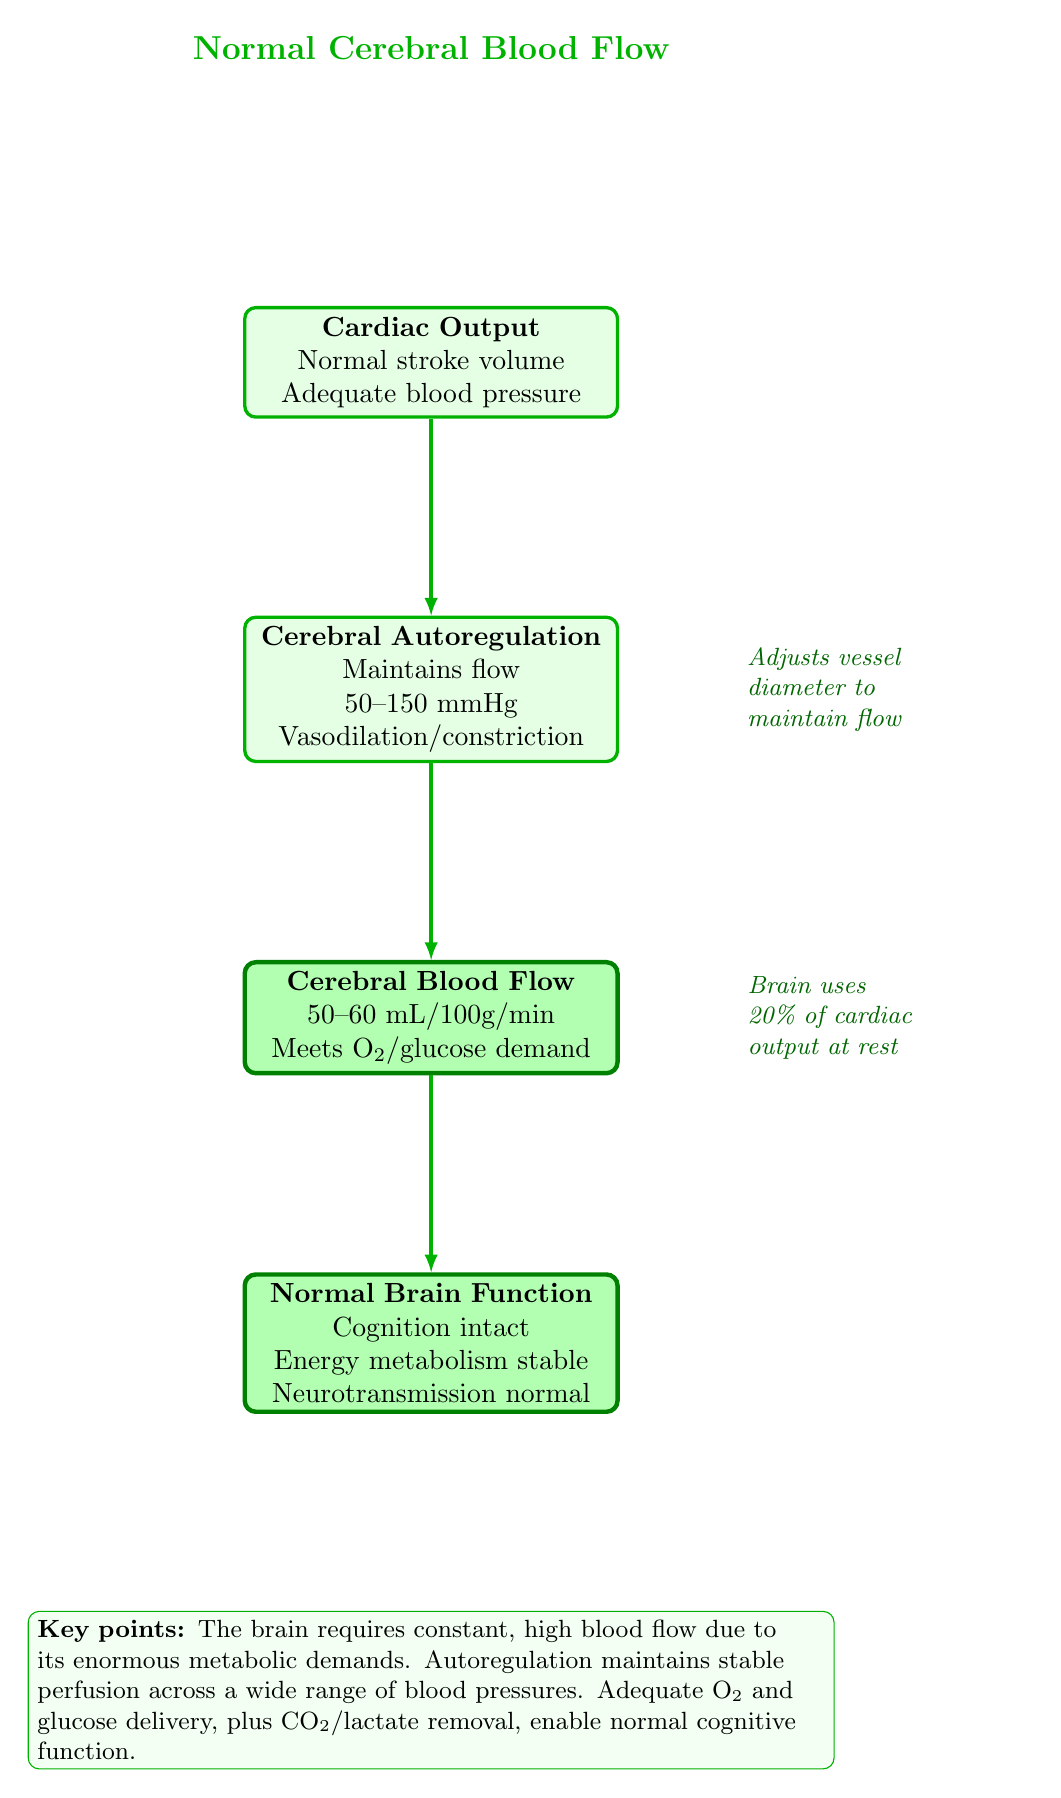
\begin{tikzpicture}[
    node distance=2.5cm,  % Global minimum vertical spacing
    % Styles
    process/.style={draw=green!70!black, fill=green!10, very thick, rounded corners, text width=4.5cm, align=center, minimum height=1.2cm},
    output/.style={draw=green!50!black, fill=green!30, ultra thick, rounded corners, text width=4.5cm, align=center, minimum height=1.3cm},
    arrow/.style={-latex, very thick, green!70!black, line width=1.2pt},
    note/.style={font=\small\itshape, text width=3.5cm, align=left, green!40!black},
]

% Title
\node[font=\large\bfseries, green!70!black] (title) at (0, 0) {Normal Cerebral Blood Flow};

% Cardiac output
\node[process, below=3cm of title] (cardiac) {\textbf{Cardiac Output}\\Normal stroke volume\\Adequate blood pressure};

% Cerebral autoregulation
\node[process, below=of cardiac] (autoreg) {\textbf{Cerebral Autoregulation}\\Maintains flow 50--150 mmHg\\Vasodilation/constriction};
\draw[arrow] (cardiac) -- (autoreg);
\node[note, right=1.5cm of autoreg] {Adjusts vessel\\diameter to\\maintain flow};

% Normal CBF
\node[output, below=of autoreg] (cbf) {\textbf{Cerebral Blood Flow}\\50--60 mL/100g/min\\Meets O\textsubscript{2}/glucose demand};
\draw[arrow] (autoreg) -- (cbf);
\node[note, right=1.5cm of cbf] {Brain uses\\20\% of cardiac\\output at rest};

% Brain function
\node[output, below=of cbf] (brain) {\textbf{Normal Brain Function}\\Cognition intact\\Energy metabolism stable\\Neurotransmission normal};
\draw[arrow] (cbf) -- (brain);

% Key point box
\node[draw=green!70!black, fill=green!5, rounded corners, text width=10cm, align=left, font=\small, below=2.5cm of brain] {
\textbf{Key points:} The brain requires constant, high blood flow due to its enormous metabolic demands. Autoregulation maintains stable perfusion across a wide range of blood pressures. Adequate O\textsubscript{2} and glucose delivery, plus CO\textsubscript{2}/lactate removal, enable normal cognitive function.
};

\end{tikzpicture}
\caption{Normal cerebral blood flow regulation meeting brain metabolic demands.}
\label{fig:cerebral-hypoperfusion-normal}
\end{figure}

\clearpage
% Figure: Cerebral Hypoperfusion in ME/CFS
% Reduced blood flow causes brain energy crisis

\begin{figure}[htbp]
\centering
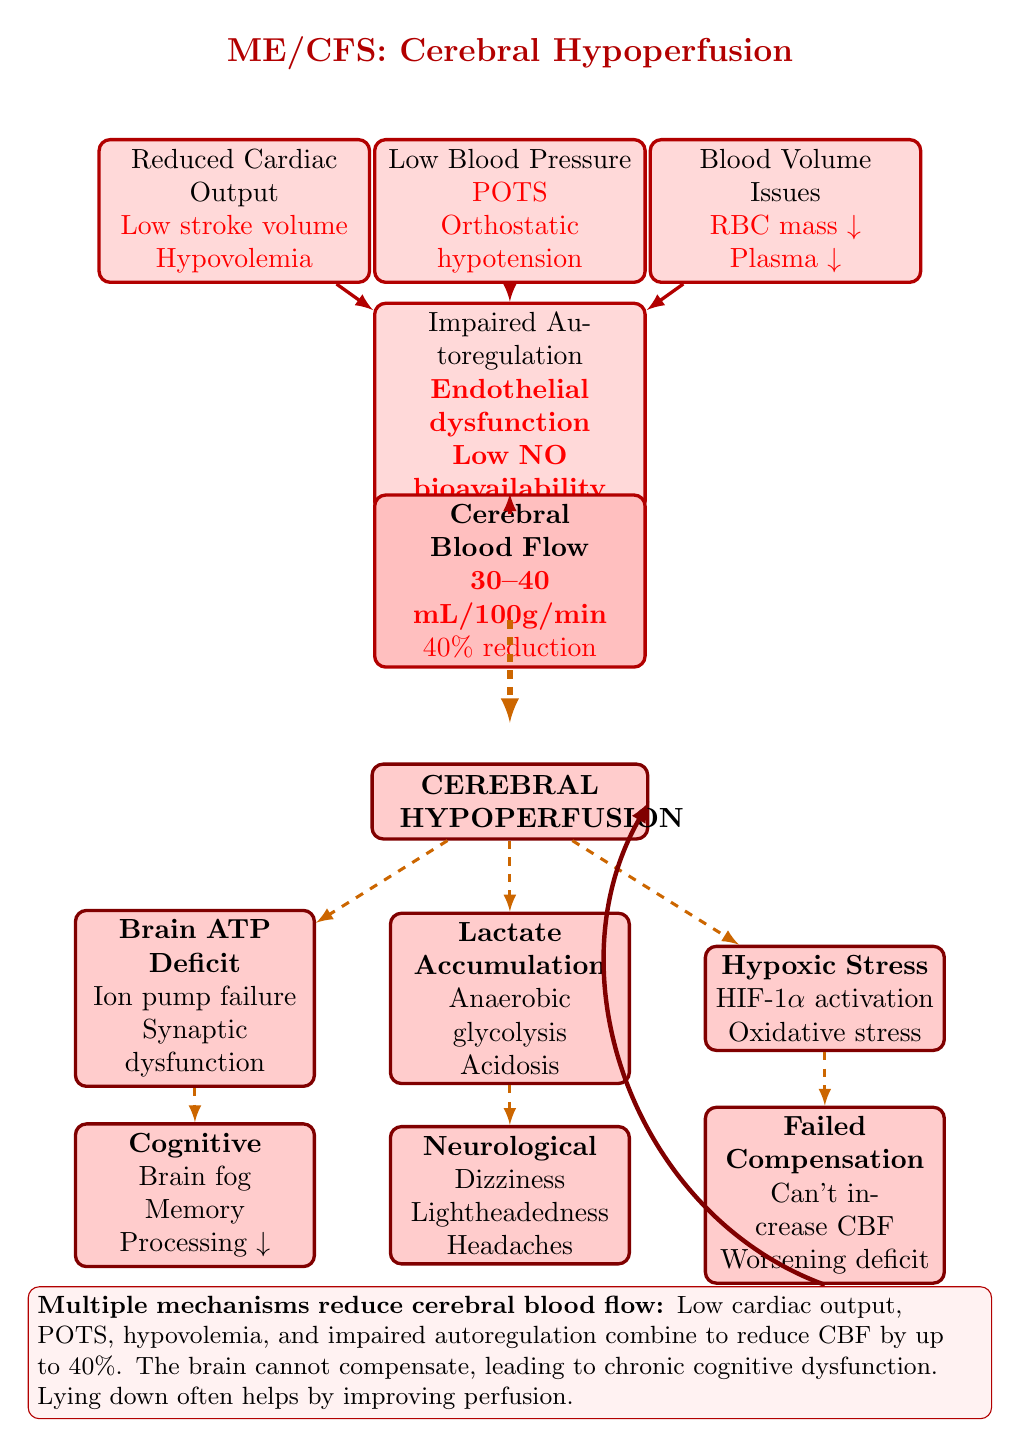
\begin{tikzpicture}[scale=1, every node/.style={scale=1},
    % Styles
    normal/.style={draw=green!70!black, fill=green!10, very thick, rounded corners, text width=3cm, align=center, minimum height=1cm},
    impaired/.style={draw=red!70!black, fill=red!15, very thick, rounded corners, text width=3.2cm, align=center, minimum height=1cm},
    severe/.style={draw=red!50!black, fill=red!25, ultra thick, rounded corners, text width=3.2cm, align=center, minimum height=1.1cm, drop shadow},
    pathological/.style={draw=red!50!black, fill=red!20, very thick, rounded corners, text width=2.8cm, align=center, minimum height=0.95cm},
    impaired-arrow/.style={-latex, very thick, red!70!black, line width=1.2pt},
    cascade-arrow/.style={-latex, thick, orange!80!black, dashed, line width=1.1pt},
    cycle-arrow/.style={-latex, ultra thick, red!50!black, line width=1.6pt},
    note/.style={font=\small\itshape, text width=2.4cm, align=left, red!60!black},
]

% Title
\node[font=\large\bfseries, red!70!black] at (0, 9) {ME/CFS: Cerebral Hypoperfusion};

% TOP: Impaired flow pathway
\begin{scope}[yshift=4.5cm]
    % Multiple contributors
    \node[impaired] (cardiac) at (-3.5, 2.5) {Reduced Cardiac\\Output\\{\color{red}Low stroke volume}\\{\color{red}Hypovolemia}};

    \node[impaired] (bp) at (0, 2.5) {Low Blood Pressure\\{\color{red}POTS}\\{\color{red}Orthostatic\\hypotension}};

    \node[impaired] (volume) at (3.5, 2.5) {Blood Volume\\Issues\\{\color{red}RBC mass $\downarrow$}\\{\color{red}Plasma $\downarrow$}};

    % Impaired autoregulation
    \node[impaired] (autoreg) at (0, 0) {Impaired Autoregulation\\{\color{red}\textbf{Endothelial dysfunction}}\\{\color{red}\textbf{Low NO bioavailability}}};
    \draw[impaired-arrow] (cardiac) -- (autoreg);
    \draw[impaired-arrow] (bp) -- (autoreg);
    \draw[impaired-arrow] (volume) -- (autoreg);

    % Reduced CBF
    \node[impaired, fill=red!25] (cbf) at (0, -2.2) {\textbf{Cerebral Blood Flow}\\{\color{red}\textbf{30--40 mL/100g/min}}\\{\color{red}40\% reduction}};
    \draw[impaired-arrow] (autoreg) -- (cbf);
\end{scope}

% BOTTOM: Cascade consequences
\begin{scope}[yshift=-3.5cm]
    % Central hypoperfusion
    \node[pathological, minimum width=3.5cm] (hypoperf) at (0, 3) {\textbf{CEREBRAL}\\  \textbf{HYPOPERFUSION}};

    % Three immediate consequences
    \node[pathological] (atp) at (-4, 0.5) {\textbf{Brain ATP}\\  \textbf{Deficit}\\Ion pump failure\\Synaptic dysfunction};

    \node[pathological] (lactate) at (0, 0.5) {\textbf{Lactate}\\  \textbf{Accumulation}\\Anaerobic glycolysis\\Acidosis};

    \node[pathological] (hypoxia) at (4, 0.5) {\textbf{Hypoxic Stress}\\HIF-1$\alpha$ activation\\Oxidative stress};

    \draw[cascade-arrow] (hypoperf) -- (atp);
    \draw[cascade-arrow] (hypoperf) -- (lactate);
    \draw[cascade-arrow] (hypoperf) -- (hypoxia);

    % Downstream symptoms
    \node[pathological] (cognitive) at (-4, -2) {\textbf{Cognitive}\\Brain fog\\Memory\\Processing $\downarrow$};

    \node[pathological] (neuro) at (0, -2) {\textbf{Neurological}\\Dizziness\\Lightheadedness\\Headaches};

    \node[pathological] (failed) at (4, -2) {\textbf{Failed}\\  \textbf{Compensation}\\Can't increase CBF\\Worsening deficit};

    \draw[cascade-arrow] (atp) -- (cognitive);
    \draw[cascade-arrow] (lactate) -- (neuro);
    \draw[cascade-arrow] (hypoxia) -- (failed);

    % Feedback loop
    \draw[cycle-arrow, bend left=50] (failed.south) to (hypoperf.east);
\end{scope}

% Arrow connecting top to bottom
\draw[cascade-arrow, line width=2pt] (0, 1.8) -- (0, 0.5);

% Key point box
\node[draw=red!70!black, fill=red!5, rounded corners, text width=12cm, align=left, font=\small] at (0, -7.5) {
\textbf{Multiple mechanisms reduce cerebral blood flow:} Low cardiac output, POTS, hypovolemia, and impaired autoregulation combine to reduce CBF by up to 40\%. The brain cannot compensate, leading to chronic cognitive dysfunction. Lying down often helps by improving perfusion.
};

\end{tikzpicture}
\caption{ME/CFS cerebral hypoperfusion cascade causing cognitive dysfunction.}
\label{fig:cerebral-hypoperfusion-mecfs}
\end{figure}

\clearpage

% Catecholamine
% Figure: Normal Catecholamine Synthesis
% Efficient production of norepinephrine and epinephrine from tyrosine

\begin{figure}[htbp]
\centering
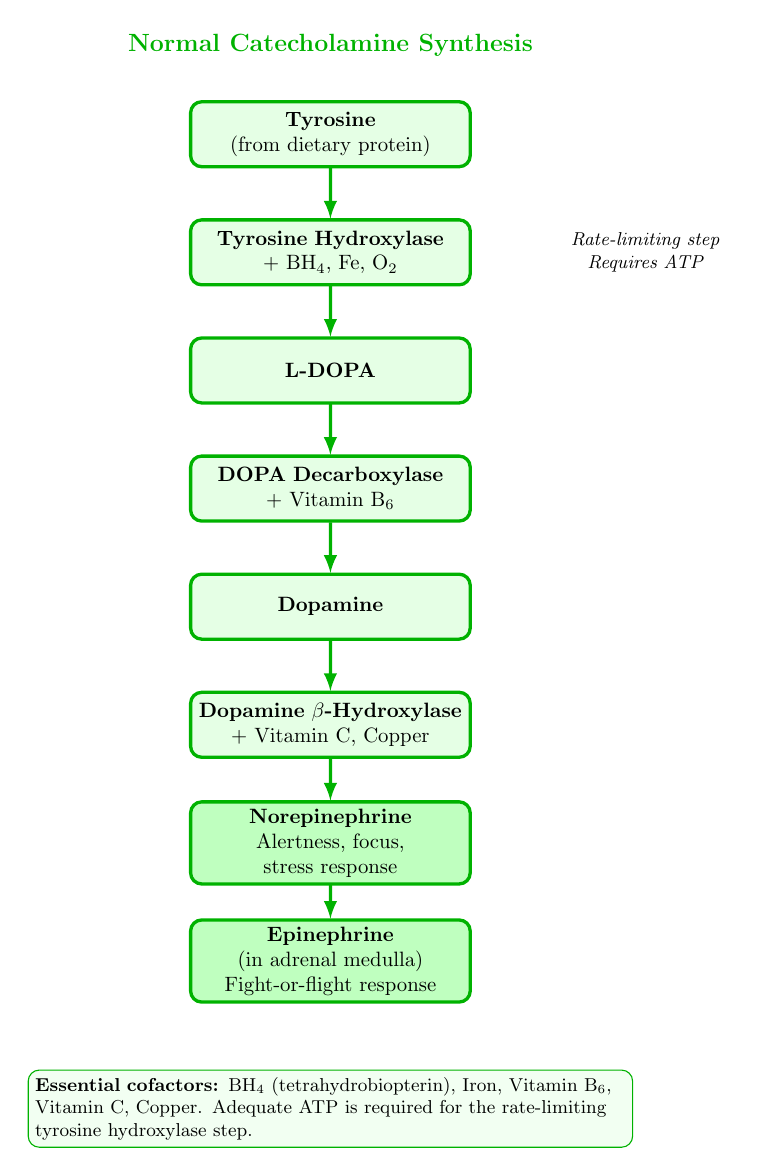
\begin{tikzpicture}[scale=0.75, every node/.style={scale=0.75},
    % Styles
    process/.style={draw=green!70!black, fill=green!10, very thick, rounded corners, text width=4.5cm, align=center, minimum height=1.1cm},
    output/.style={draw=green!70!black, fill=green!25, very thick, rounded corners, text width=4.5cm, align=center, minimum height=1.1cm},
    arrow/.style={-latex, very thick, green!70!black},
    note/.style={font=\small\itshape, text width=3.5cm, align=center},
]

% Title
\node[font=\large\bfseries, green!70!black] at (0, 9.5) {Normal Catecholamine Synthesis};

% Tyrosine
\node[process] (tyrosine) at (0, 8) {\textbf{Tyrosine}\\(from dietary protein)};

% Step 1: Tyrosine hydroxylase
\node[process] (th) at (0, 6) {\textbf{Tyrosine Hydroxylase}\\+ BH\textsubscript{4}, Fe, O\textsubscript{2}};
\draw[arrow] (tyrosine) -- (th);
\node[note, right=0.8cm of th] {Rate-limiting step\\Requires ATP};

% L-DOPA
\node[process] (ldopa) at (0, 4) {\textbf{L-DOPA}};
\draw[arrow] (th) -- (ldopa);

% Step 2: DOPA decarboxylase
\node[process] (ddc) at (0, 2) {\textbf{DOPA Decarboxylase}\\+ Vitamin B\textsubscript{6}};
\draw[arrow] (ldopa) -- (ddc);

% Dopamine
\node[process] (dopamine) at (0, 0) {\textbf{Dopamine}};
\draw[arrow] (ddc) -- (dopamine);

% Step 3: Dopamine beta-hydroxylase
\node[process] (dbh) at (0, -2) {\textbf{Dopamine $\beta$-Hydroxylase}\\+ Vitamin C, Copper};
\draw[arrow] (dopamine) -- (dbh);

% Norepinephrine
\node[output] (ne) at (0, -4) {\textbf{Norepinephrine}\\Alertness, focus, stress response};
\draw[arrow] (dbh) -- (ne);

% Epinephrine (optional path)
\node[output] (epi) at (0, -6) {\textbf{Epinephrine}\\(in adrenal medulla)\\Fight-or-flight response};
\draw[arrow] (ne) -- (epi);

% Key cofactors summary
\node[draw=green!70!black, fill=green!5, rounded corners, text width=10cm, align=left, font=\small] at (0, -8.5) {
\textbf{Essential cofactors:} BH\textsubscript{4} (tetrahydrobiopterin), Iron, Vitamin B\textsubscript{6}, Vitamin C, Copper. Adequate ATP is required for the rate-limiting tyrosine hydroxylase step.
};

\end{tikzpicture}
\caption{Normal catecholamine synthesis pathway from tyrosine to norepinephrine and epinephrine.}
\label{fig:catecholamine-normal}
\end{figure}

\clearpage
% Figure: Catecholamine Synthesis Failure in ME/CFS
% Multiple bottlenecks reduce norepinephrine/epinephrine production

\begin{figure}[htbp]
\centering
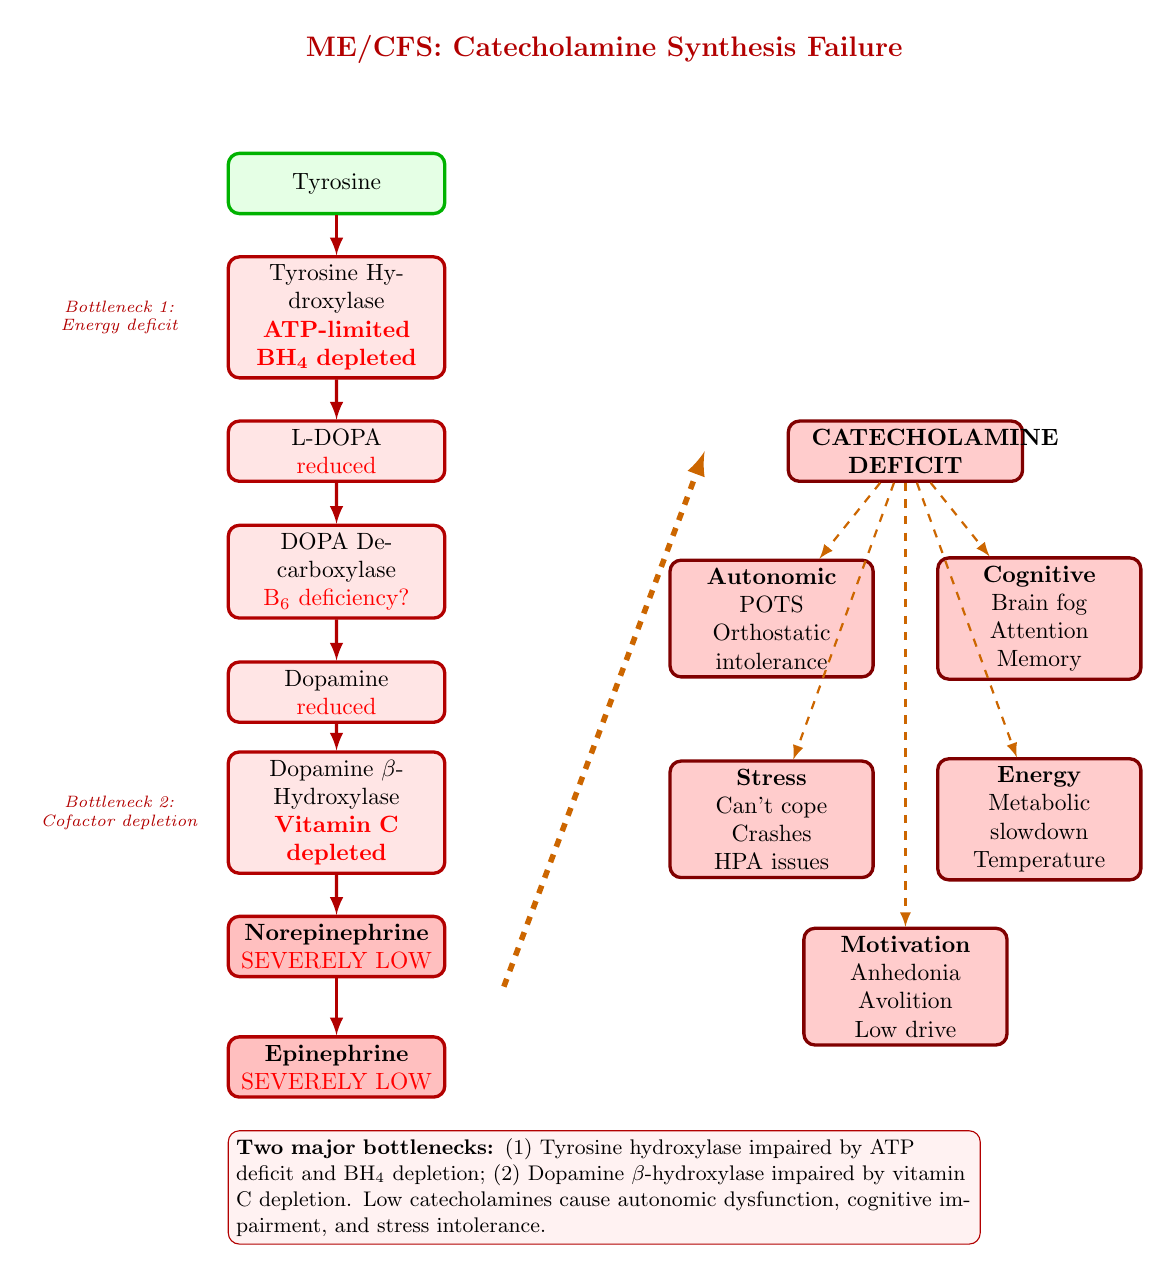
\begin{tikzpicture}[
    node distance=2.5cm,
    scale=0.85, every node/.style={scale=0.85},
    % Styles
    normal/.style={draw=green!70!black, fill=green!10, very thick, rounded corners, text width=3cm, align=center, minimum height=0.9cm},
    impaired/.style={draw=red!70!black, fill=red!10, very thick, rounded corners, text width=3cm, align=center, minimum height=0.9cm},
    pathological/.style={draw=red!50!black, fill=red!20, very thick, rounded corners, text width=2.8cm, align=center, minimum height=0.9cm},
    arrow/.style={-latex, very thick, green!70!black},
    impaired-arrow/.style={-latex, very thick, red!70!black},
    cascade-arrow/.style={-latex, thick, orange!80!black, dashed},
    note/.style={font=\scriptsize\itshape, text width=2.5cm, align=center},
]

% Title
\node[font=\large\bfseries, red!70!black] at (0, 9) {ME/CFS: Catecholamine Synthesis Failure};

% LEFT SIDE: Impaired pathway
\begin{scope}[xshift=-4cm]
    % Tyrosine (normal)
    \node[normal] (tyrosine) at (0, 7) {Tyrosine};

    % Bottleneck 1: TH impaired
    \node[impaired] (th) at (0, 5) {Tyrosine Hydroxylase\\{\color{red}\textbf{ATP-limited}}\\{\color{red}\textbf{BH\textsubscript{4} depleted}}};
    \draw[impaired-arrow] (tyrosine) -- (th);
    \node[note, left=0.2cm of th, text=red!70!black] {Bottleneck 1:\\Energy deficit};

    % L-DOPA (reduced)
    \node[impaired] (ldopa) at (0, 3) {L-DOPA\\{\color{red}reduced}};
    \draw[impaired-arrow] (th) -- (ldopa);

    % DDC (may be impaired)
    \node[impaired] (ddc) at (0, 1.2) {DOPA Decarboxylase\\{\color{red}B\textsubscript{6} deficiency?}};
    \draw[impaired-arrow] (ldopa) -- (ddc);

    % Dopamine (reduced)
    \node[impaired] (dopamine) at (0, -0.6) {Dopamine\\{\color{red}reduced}};
    \draw[impaired-arrow] (ddc) -- (dopamine);

    % Bottleneck 2: DBH impaired
    \node[impaired] (dbh) at (0, -2.4) {Dopamine $\beta$-Hydroxylase\\{\color{red}\textbf{Vitamin C depleted}}};
    \draw[impaired-arrow] (dopamine) -- (dbh);
    \node[note, left=0.2cm of dbh, text=red!70!black] {Bottleneck 2:\\Cofactor depletion};

    % Severely reduced outputs
    \node[impaired, fill=red!25] (ne) at (0, -4.4) {\textbf{Norepinephrine}\\{\color{red}SEVERELY LOW}};
    \draw[impaired-arrow] (dbh) -- (ne);

    \node[impaired, fill=red!25] (epi) at (0, -6.2) {\textbf{Epinephrine}\\{\color{red}SEVERELY LOW}};
    \draw[impaired-arrow] (ne) -- (epi);
\end{scope}

% RIGHT SIDE: System failures
\begin{scope}[xshift=4.5cm]
    % Central deficit
    \node[pathological, minimum width=3.5cm] (deficit) at (0, 3) {\textbf{CATECHOLAMINE}\\  \textbf{DEFICIT}};

    % Five consequences
    \node[pathological] (autonomic) at (-2, 0.5) {\textbf{Autonomic}\\POTS\\Orthostatic\\intolerance};

    \node[pathological] (cognitive) at (2, 0.5) {\textbf{Cognitive}\\Brain fog\\Attention\\Memory};

    \node[pathological] (stress) at (-2, -2.5) {\textbf{Stress}\\Can't cope\\Crashes\\HPA issues};

    \node[pathological] (energy) at (2, -2.5) {\textbf{Energy}\\Metabolic\\slowdown\\Temperature};

    \node[pathological] (motivation) at (0, -5) {\textbf{Motivation}\\Anhedonia\\Avolition\\Low drive};

    % Cascade arrows
    \draw[cascade-arrow] (deficit) -- (autonomic);
    \draw[cascade-arrow] (deficit) -- (cognitive);
    \draw[cascade-arrow] (deficit) -- (stress);
    \draw[cascade-arrow] (deficit) -- (energy);
    \draw[cascade-arrow] (deficit) -- (motivation);
\end{scope}

% Arrow connecting left to right
\draw[cascade-arrow, line width=2pt] (-1.5, -5) -- (1.5, 3);

% Key point box
\node[draw=red!70!black, fill=red!5, rounded corners, text width=11cm, align=left, font=\small] at (0, -8) {
\textbf{Two major bottlenecks:} (1) Tyrosine hydroxylase impaired by ATP deficit and BH\textsubscript{4} depletion; (2) Dopamine $\beta$-hydroxylase impaired by vitamin C depletion. Low catecholamines cause autonomic dysfunction, cognitive impairment, and stress intolerance.
};

\end{tikzpicture}
\caption{ME/CFS catecholamine synthesis failure and systemic consequences.}
\label{fig:catecholamine-mecfs}
\end{figure}

\clearpage

% Tryptophan
% Figure: Normal Tryptophan Metabolism
% Balanced split between serotonin and kynurenine pathways

\begin{figure}[htbp]
\centering
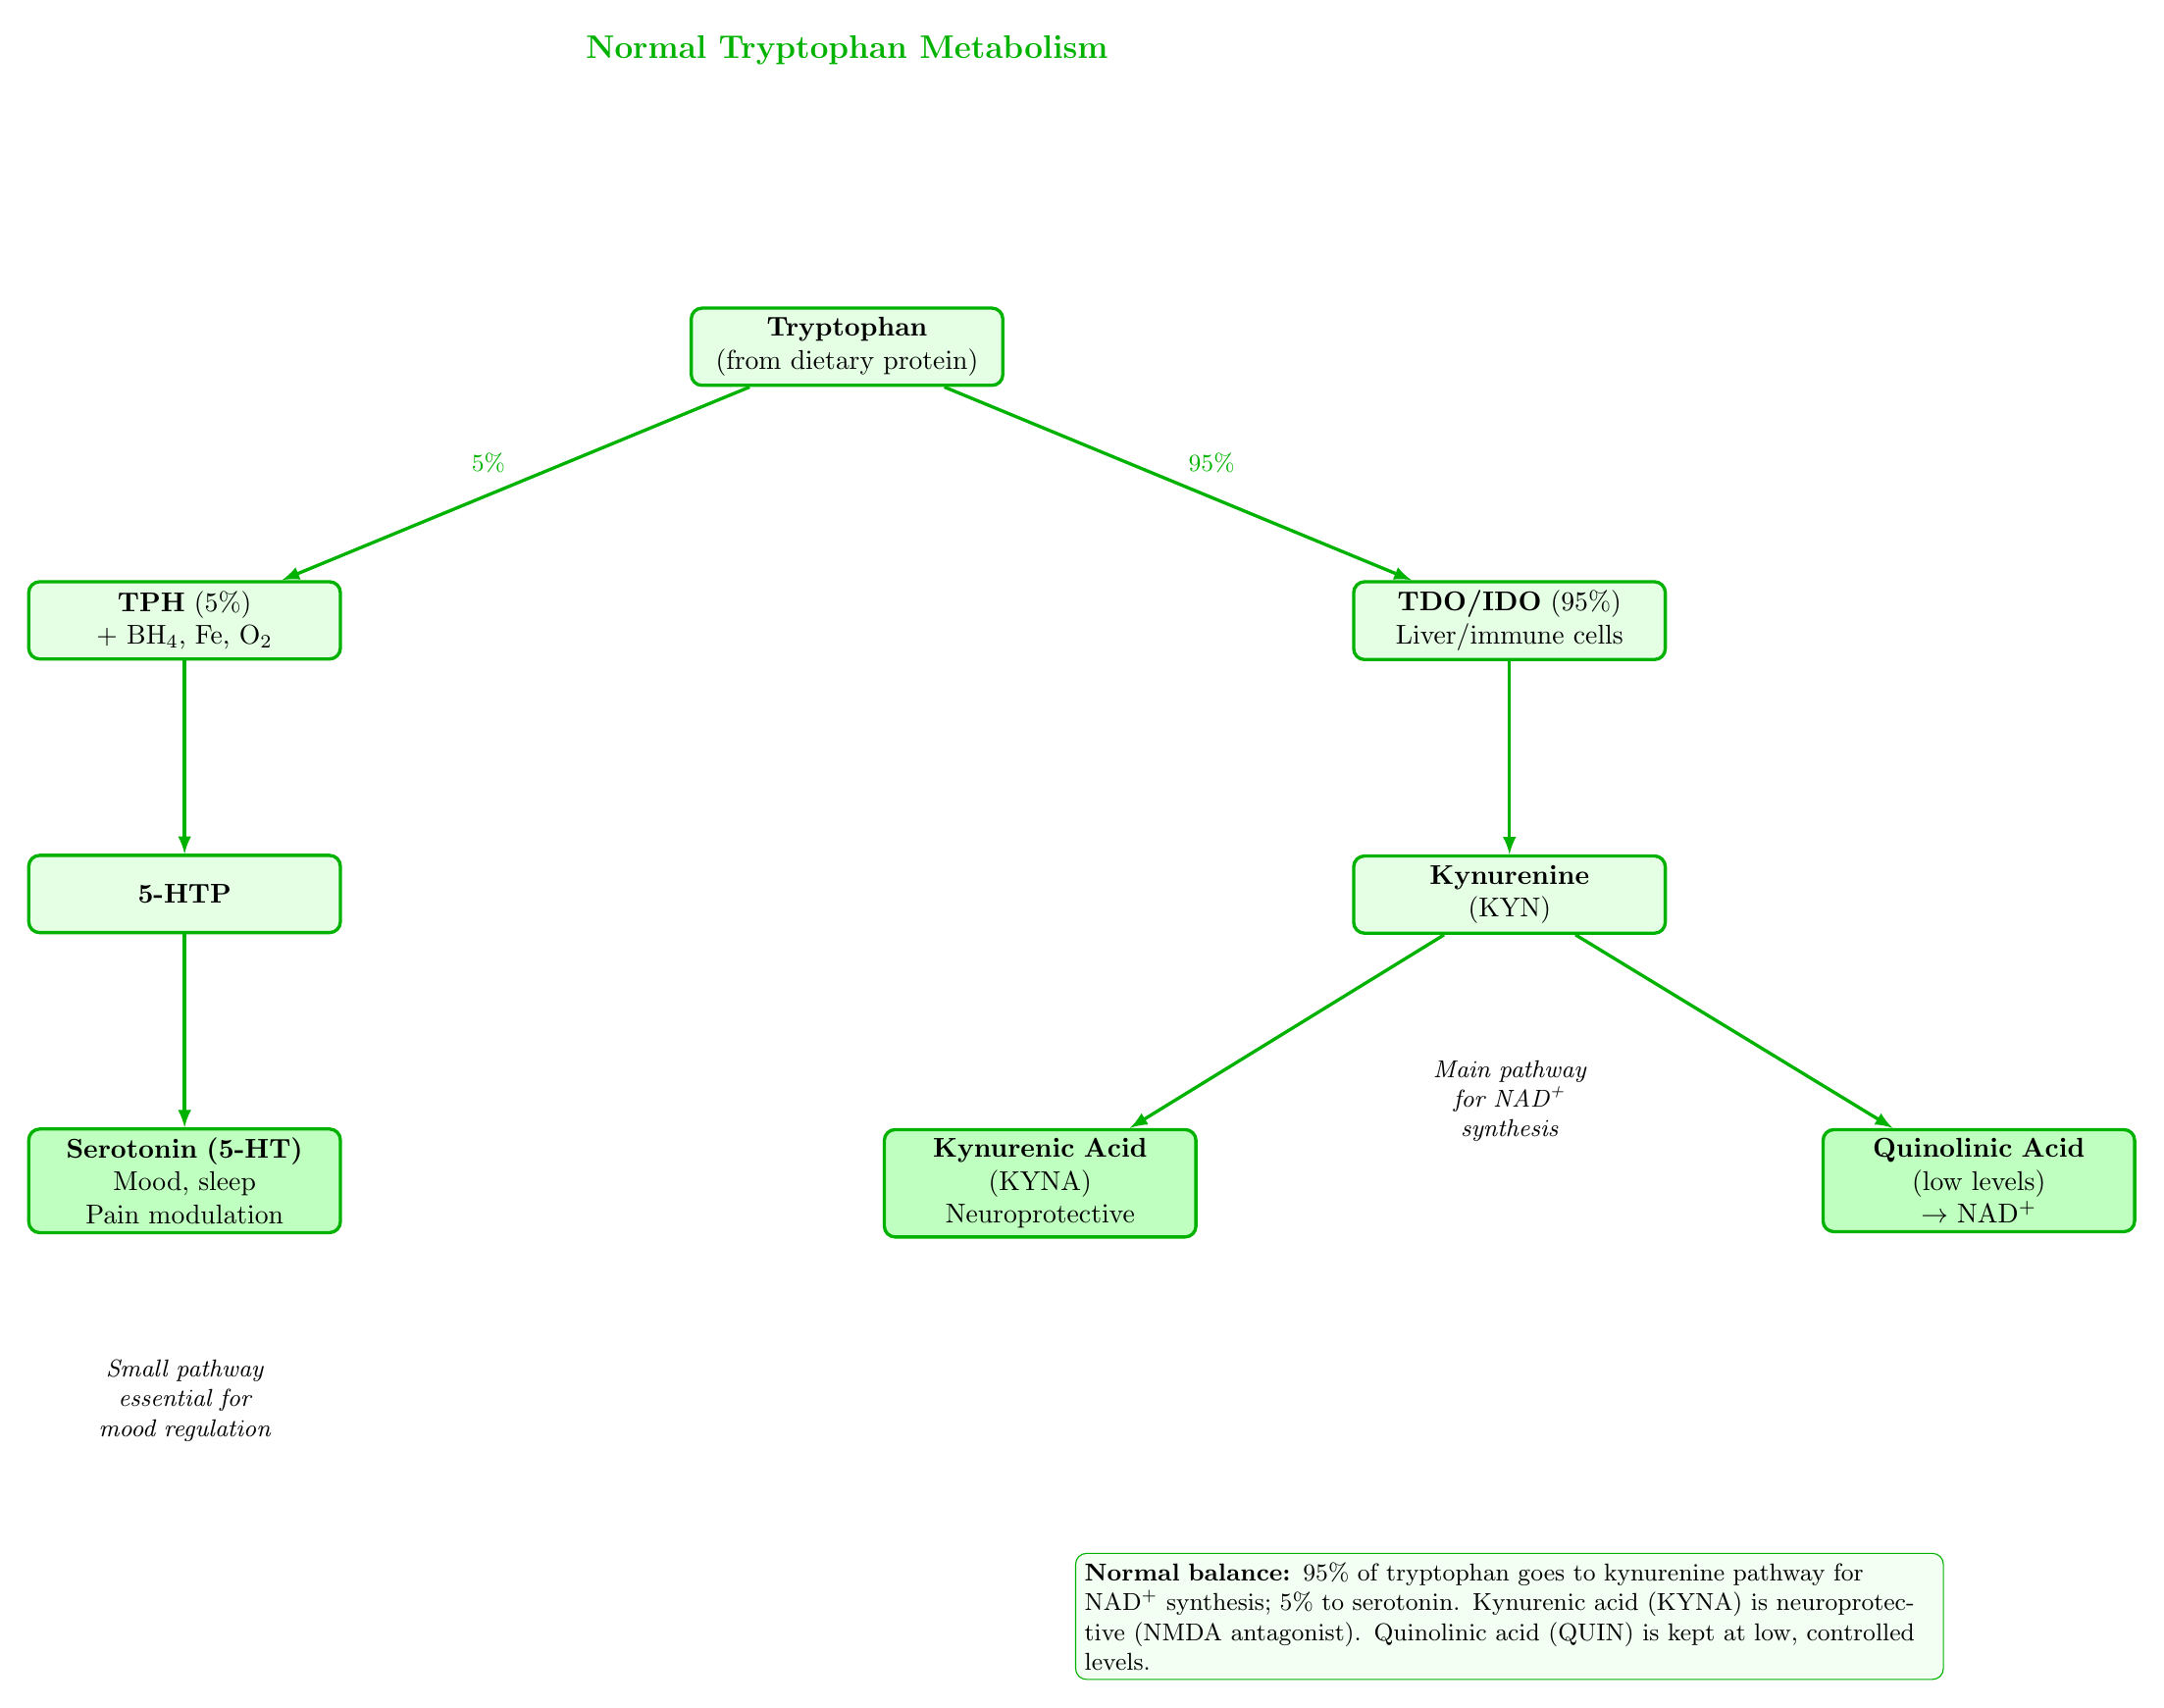
\begin{tikzpicture}[
    node distance=2.5cm and 4cm,  % Vertical and horizontal spacing
    % Styles
    process/.style={draw=green!70!black, fill=green!10, very thick, rounded corners, text width=3.8cm, align=center, minimum height=1cm},
    output/.style={draw=green!70!black, fill=green!25, very thick, rounded corners, text width=3.8cm, align=center, minimum height=1cm},
    arrow/.style={-latex, very thick, green!70!black},
    note/.style={font=\small\itshape, text width=3cm, align=center},
]

% Title
\node[font=\large\bfseries, green!70!black] (title) at (0, 0) {Normal Tryptophan Metabolism};

% Tryptophan input
\node[process, below=3cm of title] (trp) {\textbf{Tryptophan}\\(from dietary protein)};

% LEFT BRANCH: Serotonin pathway (5%)
\node[process, below left=2.5cm and 4.5cm of trp] (tph) {\textbf{TPH} (5\%)\\+ BH\textsubscript{4}, Fe, O\textsubscript{2}};
\draw[arrow] (trp) -- node[above left, font=\small] {5\%} (tph);

\node[process, below=of tph] (fivehttp) {\textbf{5-HTP}};
\draw[arrow] (tph) -- (fivehttp);

\node[output, below=of fivehttp] (serotonin) {\textbf{Serotonin (5-HT)}\\Mood, sleep\\Pain modulation};
\draw[arrow] (fivehttp) -- (serotonin);

% RIGHT BRANCH: Kynurenine pathway (95%)
\node[process, below right=2.5cm and 4.5cm of trp] (tdo) {\textbf{TDO/IDO} (95\%)\\Liver/immune cells};
\draw[arrow] (trp) -- node[above right, font=\small] {95\%} (tdo);

\node[process, below=of tdo] (kyn) {\textbf{Kynurenine}\\(KYN)};
\draw[arrow] (tdo) -- (kyn);

% Kynurenine splits
\node[output, below left=2.5cm and 2cm of kyn] (kyna) {\textbf{Kynurenic Acid}\\(KYNA)\\Neuroprotective};
\draw[arrow] (kyn) -- (kyna);

\node[output, below right=2.5cm and 2cm of kyn] (quin) {\textbf{Quinolinic Acid}\\(low levels)\\$\rightarrow$ NAD\textsuperscript{+}};
\draw[arrow] (kyn) -- (quin);

% Notes
\node[note, below=1.5cm of serotonin] {Small pathway\\essential for\\mood regulation};
\node[note, below=1.5cm of kyn] {Main pathway\\for NAD\textsuperscript{+}\\synthesis};

% Key point box
\node[draw=green!70!black, fill=green!5, rounded corners, text width=11cm, align=left, font=\small, below=8cm of kyn] {
\textbf{Normal balance:} 95\% of tryptophan goes to kynurenine pathway for NAD\textsuperscript{+} synthesis; 5\% to serotonin. Kynurenic acid (KYNA) is neuroprotective (NMDA antagonist). Quinolinic acid (QUIN) is kept at low, controlled levels.
};

\end{tikzpicture}
\caption{Normal tryptophan metabolism with balanced serotonin and kynurenine pathways.}
\label{fig:tryptophan-normal}
\end{figure}

\clearpage
% Figure: Tryptophan-Kynurenine Dysregulation in ME/CFS
% Inflammation drives tryptophan away from serotonin, toxic metabolites accumulate

\begin{figure}[htbp]
\centering
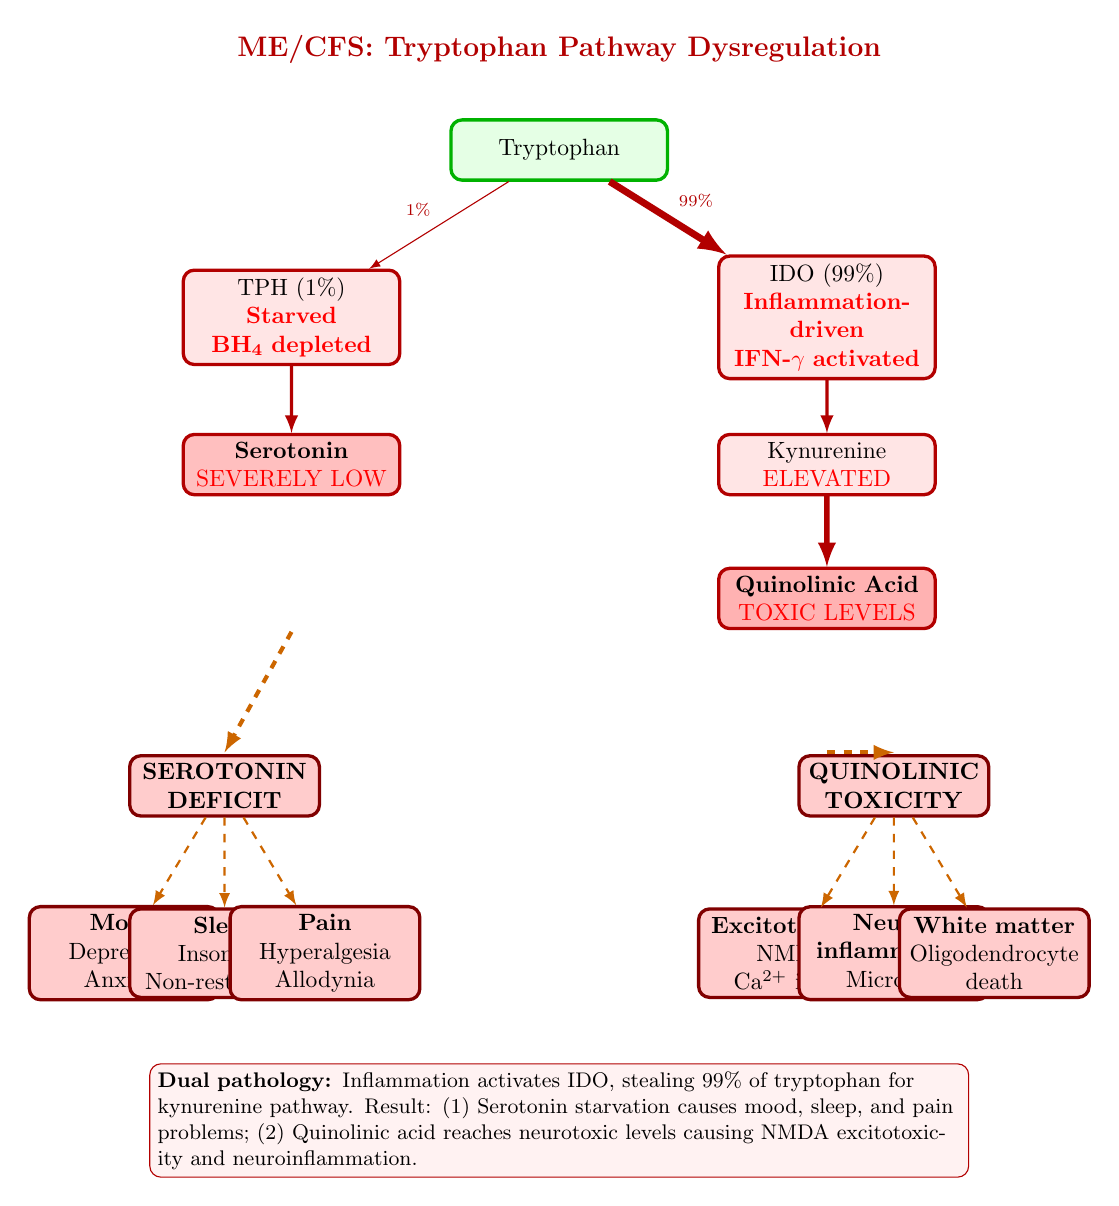
\begin{tikzpicture}[
    node distance=2.5cm,
    scale=0.85, every node/.style={scale=0.85},
    % Styles
    normal/.style={draw=green!70!black, fill=green!10, very thick, rounded corners, text width=3cm, align=center, minimum height=0.9cm},
    impaired/.style={draw=red!70!black, fill=red!10, very thick, rounded corners, text width=3cm, align=center, minimum height=0.9cm},
    pathological/.style={draw=red!50!black, fill=red!20, very thick, rounded corners, text width=2.6cm, align=center, minimum height=0.9cm},
    arrow/.style={-latex, very thick, green!70!black},
    impaired-arrow/.style={-latex, very thick, red!70!black},
    cascade-arrow/.style={-latex, thick, orange!80!black, dashed},
    note/.style={font=\scriptsize\itshape, text width=2.3cm, align=center},
]

% Title
\node[font=\large\bfseries, red!70!black] at (0, 9) {ME/CFS: Tryptophan Pathway Dysregulation};

% TOP: Dysregulated pathway
\begin{scope}[yshift=5cm]
    % Tryptophan
    \node[normal] (trp) at (0, 2.5) {Tryptophan};

    % LEFT: Serotonin - STARVED
    \node[impaired] (tph) at (-4, 0) {TPH (1\%)\\{\color{red}\textbf{Starved}}\\{\color{red}\textbf{BH\textsubscript{4} depleted}}};
    \draw[impaired-arrow, thin] (trp) -- node[above left, font=\scriptsize] {1\%} (tph);

    \node[impaired, fill=red!25] (serotonin) at (-4, -2.2) {\textbf{Serotonin}\\{\color{red}SEVERELY LOW}};
    \draw[impaired-arrow] (tph) -- (serotonin);

    % RIGHT: Kynurenine - HYPERACTIVE
    \node[impaired] (ido) at (4, 0) {IDO (99\%)\\{\color{red}\textbf{Inflammation-driven}}\\{\color{red}\textbf{IFN-$\gamma$ activated}}};
    \draw[impaired-arrow, line width=2.5pt] (trp) -- node[above right, font=\scriptsize] {99\%} (ido);

    \node[impaired] (kyn) at (4, -2.2) {Kynurenine\\{\color{red}ELEVATED}};
    \draw[impaired-arrow] (ido) -- (kyn);

    % Quinolinic acid - TOXIC
    \node[impaired, fill=red!30] (quin) at (4, -4.2) {\textbf{Quinolinic Acid}\\{\color{red}TOXIC LEVELS}};
    \draw[impaired-arrow, line width=2pt] (kyn) -- (quin);
\end{scope}

% BOTTOM: Dual pathology consequences
\begin{scope}[yshift=-4cm]
    % Serotonin deficit consequences (left)
    \node[pathological] (sero-def) at (-5, 2) {\textbf{SEROTONIN}\\  \textbf{DEFICIT}};

    \node[pathological] (mood) at (-6.5, -0.5) {\textbf{Mood}\\Depression\\Anxiety};
    \node[pathological] (sleep) at (-5, -0.5) {\textbf{Sleep}\\Insomnia\\Non-restorative};
    \node[pathological] (pain) at (-3.5, -0.5) {\textbf{Pain}\\Hyperalgesia\\Allodynia};

    \draw[cascade-arrow] (sero-def) -- (mood);
    \draw[cascade-arrow] (sero-def) -- (sleep);
    \draw[cascade-arrow] (sero-def) -- (pain);

    % Quinolinic acid consequences (right)
    \node[pathological] (quin-tox) at (5, 2) {\textbf{QUINOLINIC}\\  \textbf{TOXICITY}};

    \node[pathological] (excito) at (3.5, -0.5) {\textbf{Excitotoxicity}\\NMDA\\Ca\textsuperscript{2+} influx};
    \node[pathological] (neuroinf) at (5, -0.5) {\textbf{Neuro-}\\  \textbf{inflammation}\\Microglia};
    \node[pathological] (white) at (6.5, -0.5) {\textbf{White matter}\\Oligodendrocyte\\death};

    \draw[cascade-arrow] (quin-tox) -- (excito);
    \draw[cascade-arrow] (quin-tox) -- (neuroinf);
    \draw[cascade-arrow] (quin-tox) -- (white);
\end{scope}

% Arrows from pathway to consequences
\draw[cascade-arrow, line width=1.5pt] (-4, 0.3) -- (-5, -1.5);
\draw[cascade-arrow, line width=1.5pt] (4, -1.5) -- (5, -1.5);

% Key point box
\node[draw=red!70!black, fill=red!5, rounded corners, text width=12cm, align=left, font=\small] at (0, -7) {
\textbf{Dual pathology:} Inflammation activates IDO, stealing 99\% of tryptophan for kynurenine pathway. Result: (1) Serotonin starvation causes mood, sleep, and pain problems; (2) Quinolinic acid reaches neurotoxic levels causing NMDA excitotoxicity and neuroinflammation.
};

\end{tikzpicture}
\caption{ME/CFS tryptophan dysregulation causing serotonin deficit and quinolinic acid toxicity.}
\label{fig:tryptophan-mecfs}
\end{figure}


\end{document}
